\documentclass[12pt]{report}

\usepackage[top=2cm,bottom=2cm,left=2cm,right=2cm]{geometry}
\usepackage[pdftex]{graphicx} 
\usepackage[utf8]{inputenc}   
\usepackage[english]{babel}
\usepackage{amsthm}
\usepackage{dsfont} % for the R of real
\usepackage{physics}
\usepackage{bm} % for a textbf in math mode
\usepackage{tcolorbox} %for boxes of text/math


\theoremstyle{plain}
\newtheorem{theorem}{Theorem}[chapter]
\newtheorem{definition}{Definition}[chapter]
\newtheorem{proposition}{Proposition}[chapter]
\newtheorem{lemma}{Lemma}[chapter]
\newtheorem{example}{Example}[chapter]
\newtheorem{corollary}{Corollary}[theorem]

\newcommand\mcl[1]{\mathcal{#1}}
\newcommand\sprod[2]{\langle \vb{#1},\vb{#2}\rangle}

\begin{document}
\begin{flushleft}
	
	\begin{center}
		\begin{figure}
			\centering
			
\includegraphics[scale=.13]{images/logo_unipd.png}
		\end{figure}
		Università degli studi di Padova\\
		Dipartimento di Fisica “Galileo Galilei”\\
		Academic year 2019/2020\\

		\vspace{1cm}		
		\large{\textit{Master degree in Physics of Data}}\\
		\vspace{1cm}
		\huge{\textbf{Notes of Machine Learning}}
	\end{center}
	
\tableofcontents


\chapter*{What is Machine Learning?}
The main subject o these notes is automated learning, or, as we will more often call it, Machine Learning (ML). Machine Learning is essentially "teaching to the computers so they can learn from inputs we give them". The input to a learning algorithm is training data, representing experience, and the output is some expertise, usually a new program that can independently perform a task.\\
A tipical example of a learning algorithm is a program that can distnguish between male and female people: it will be trained with a sample of different people (more heterogeneous as possible) to teach it the main differences of the two genres.\\
Another example is an algorithm that gives the probability of a person to have a certain height given, for example, the genre or the age.\\
A more common example is the algorithm that, between emails, can distinguish spam emails from the other ones.\\
Before starting the effective lectures, we should define a first small difference between the types of learning: 
since learning involves an interaction between the learner and the environment, one can divide learning tasks according to the nature of that interaction.  
\begin{itemize}
\item \textit{Supervised learning} describes a scenario in which the "experience", the training data, contains significant information that is missing in the unseen “test examples” to which the learned expertise is to be applied. In this setting, the acquired expertise is aimed to predict that missing information for the test data. In such cases, we can think of the environment as a teacher that “supervises” the learner by providing the extra information (labels). More abstractly, the algorithm can be seen as a process of "using experience to gain experties".
\item In \textit{Unsupervised learning}, instead, there is no distinction between training and test data: the learner processes input data with the goal of coming up with some summary, or compressed version of that data.
\end{itemize}


\chapter{Machine Learning Model}

First of all, we give some definitions of the stuff the machine learnig algorithm has access to:
\begin{itemize}
\item \textbf{Domain set} (or \textbf{instance space} $\mcl{X}$): is the set of all possible objects that we want to label, i.e. make prediction about. Usually this is a "vector of features".
\item \textbf{Label set}: contains all possible prediction (labels). Usually correspond to the binary set $\left\{0,1\right\}$ (that can mean $\left\{True,False\right\}$).
\item \textbf{Training data}: $S=((x_1,y_1),\dots,(x_m,y_m))$ is a finite sequence of pairs in $\mcl{X}\times \mathcal{y}$, and represent the input of the ML algorithm. The index $m$, instead, represent the dimension of the dataset. Despite the "set" notation, $S$ is a sequence. In particular, the same example may appear twice in $S$ and some algorithms can take into account the order of examples in $S$.
\item \textbf{Prediction rule}: Is a function $h:\mcl{X}\to\mcl{y}$ (also called "predictor", "hypotheses" or "classifier") that can be used to predict the label of new domain points. We denote $A(S)$ the hypothesis that a learning algorithm $A$ returns upon receiving the training sequence $S$.
\item \textbf{Data-generation model}: We assume that the instances are generated by some probability distribution $\mcl{D}$ (not known by the algorithm), and we assume that there is a "correct" labelling function $f:\mcl{X}\to\mcl{y}$ for which $y_i = f(x_i) \quad \forall i$. The labelling function isn't known by the algorithm: in fact, it is just what the program is trying to figure out. In summary, each pair in the training data is generated by first sampling a point $x_i$ according to $\mcl{D}$ and then labelling it by $f$.
\item \textbf{Measure of success}: We define \textit{error of the classifier} the probability that the algorithm does not predict the correct label on a random data point generated by distribution $\mcl{D}$. In other words, the error of $h$ i the probability to draw a random instance $x$, according to the distribution $\mcl{D}$, such that $h(x) \neq f(x)$.
\end{itemize}

Usually, our sample will be a vector (so a set of numbers) $x\in\mathds{R}^d$.\\
We must pay attention that what the algorithm learn depends on training data! So, if the training data are bad, the results will be bad aswell.

\section{Measure of Success: Loss Function}

Given a domain subset $A\subset\mcl{X}$ and the probability distribution $\mcl{D}$, $\mcl{D}(A)$ represents the probability of observing a point $x\in A$.\\
In many cases, we refer to $A$ as an \textit{event} and express it using a function $\pi :\mcl{X}\to\left\{0,1\right\}$, that is $A = \left\{x\in\mcl{X}:\pi(x)=1\right\}$.\\   
In this case denote $\mcl{D}(A)$ as $\mathds{P}_{x\sim\mcl{D}}\left[\pi(x)\right]$, where $\sim$ indicates that $x$ point is sampled according to $\mcl{D}$.\\
Now, we define the \textbf{error of prediction rule}:
\begin{equation}
\ell_{\mcl{D},f}(h) = \ell_\mcl{D}(h) = \mathds{P}_{x\sim\mcl{D}}\left[h(x)\neq f(x)\right] = \mcl{D}\left(\left\{x:h(x)\neq f(x)\right\}\right)
\label{eq:err_pred_rule}
\end{equation}
This is nothing but the probability of randomly choosing an example $x$ for which $h(x)\neq f(x)$. It is also called \textit{generalization error}, or \textbf{true error}.\\
It is important to understand that the algorithm doesn't know the probability distribution $\mcl{D}$, so it is not able to compute the true error. 

\section{Empirical Risk Minimization}

As mentioned earlier, a learning algorithm receives as input a training set $S$, sampled from an unknown distribution $\mcl{D}$ and labeled by some target function $f$, and should output a predictor $h_S:\mcl{X}\to\mcl{Y}$ (the subscript $S$ emphasizes the fact that the output predictor depends on the training set). The goal of the algorithm is to find $h_S$ that minimizes the error with respect to the unknown $\mcl{D}$ and $f$.\\
If, because of the true error can't be computed, we would like to try another estimate of it, we should define the error on the training data, called \textbf{training error}:
\begin{equation}
\ell_S(h) = \frac{\abs{i:h(x_i)\neq y_i , i=1,\dots ,m}}{m}
\label{eq:train_err}
\end{equation}
This division is simply the rate o correct prediction and the total samples (assuming classification problem and 0-1 loss), and it is also called \textit{empirical error} or \textit{empirical risk}.\\
This learning paradigm, which main goal is to find a predictor $h$ that minimize $\ell_S$, is called \textit{Empirical Risk Minimization} or ERM, for short.\\

\vspace{0.5cm}
Although the ERM rule seems very natural, without being careful this approach may fail miserabily.\\
Let's consider, for example, the sample in figure \ref{fig:overfit} (on the left), assuming a probability distribution $\mcl{D}$ for which instances $x$ are taken uniformily at random in the square, and the labelling function $f$ that assign the value 1 to the instances in the upper squares, and 0 to the others (essentially 0 to blue ones and 1 to red ones). If we collect the training set shown in figure \ref{fig:overfit} (on the right), to train the ML algorithm, a good predictor seems to be the function $h_S(x) = \left\{\begin{aligned} &0 \text{ if x in left side}\\ &1 \text{ if x in right side}\end{aligned}\right.$, that effectively minimize the training loss ($L_S(h_S) =0$, practically perfect). But is this a good predictor?

\begin{figure}[hbtp]
\centering
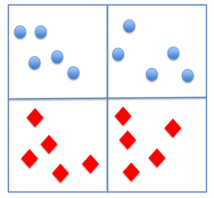
\includegraphics[scale=1.5]{images/overfit_ex_1.pdf}\qquad\qquad
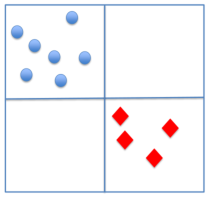
\includegraphics[scale=1.5]{images/overfit_ex_2.pdf}
\caption{Example of overfitting}
\label{fig:overfit}
\end{figure}

On the other hand, the true error of any classifier is, in this case $L_\mcl{D}(h_S) = \frac{1}{2}$.\\
We have found a predictor whose performance on the training set is excellent, yet its performance on the true “world” is very poor. This phenomenon is called overfitting. Intuitively, overfitting occurs when our hypothesis fits the training data “too well”, but doesn't have the same performances on a generic dataset. We obviously want to avoid this overfitting, because algorithms should work in general cases. Overfitting is less probable when the training set is large. The bigger is a training set, the smaller will be the probability to have regular distribution of data.\\


\section{Hypothesis class}
Rather than giving up completely the ERM paradigm, we want to look at the conditions under which it is guarantee that ERM does not overfit.\\
A common solution is to apply the ERM learning rule over a restricted search space. Formally, the learner should choose in advance (before seeing the data) a set of predictors. This set is called a \textbf{hypothesis class} and is denoted by $\mcl{H}$. Each $h\in\mcl{H}$ is a function mapping from $\mcl{X}$ to $\mcl{Y}$. For a given class $\mcl{H}$, and a training sample, $S$, the $ERM_\mcl{H}$ learner uses the ERM rule to choose a predictor $h$, with the lowest possible error over $S$:
\begin{equation}
ERM_\mcl{H} \in \underset{h\in\mcl{H`}}{argmin}\, L_S(h)
\label{eq:ERMH}
\end{equation}
where $argmin$ stands for the set of hypotheses in $\mcl{H}$ that achieve the minimum value of $L_S(h)$.\\
Since the choice of such a restriction is determined before the learner sees the training data, it should ideally be based on some prior knowledge about the problem to be learned. Intuitively, choosing a more restricted hypothesis class better protects us against overfitting but at the same time might cause us a stronger inductive bias: if the class is too small you will not find a good estimator.\\
Now we would like to prove that, if $\mcl{H}$ is a finite class $ERM_\mcl{H}$ is guarantee not to overfit, provided it is based on a sufficiently large training sample (depending on the size of $\mcl{H}$). Limiting the dimension of $\mcl{H}$ ($\abs{\mcl{H}} < \infty$) seems not to be very realistic, because we usually have to deal with parameters defined in $\mathds{R}^d$: the correct assumption uses the finite precision with which computers manage real numbers.\\
Let us now analyze the performance of the $ERM_\mcl{H}$ learning rule assuming that $\mcl{H}$ is a finite class. For a training sample, $S$, labeled according to some $f:\mcl{X}\to\mcl{Y}$, let $h_S$ denote a result of applying $ERM_\mcl{H}$ to $S$, i.e. $h_s\in \underset{h\in\mcl{H}}{argmin}\, L_S(h)$. Let's make some assumptions:
\begin{itemize}
\item (\textbf{Realizability}) There exist a $h^*\in\mcl{H}$ such that $L_\mcl{D}(h^*)=0$: in practice we are asking for the existance of the perfect solution in our hypothesis class. Note that this assumption implies that with probability 1 over random samples, we have $L_S(h^*)=0$.
\item (\textbf{i.i.d.}) The examples in the training set are indipendently and identically distributed (i.i.d.) according to the distribution $\mcl{D}$ and than labelled according the labeling function $f$. We denote this assumption by $S\sim\mcl{D}^m$ (this notation represents the fact that we sample $m$ times according to the distribution $\mcl{D}$). This assumption seems to be unrealistic too: the sampling is usually biased on the situation; you will never be able to sample reproducing the real distribution and leave them indipendent between each other. Anyway, the larger the sample get, the more likely it is to reflect more accurately the distribution ad labelig used to generate it.
\end{itemize}
Since $L_\mcl{D}(h_S)$ depends on the training set S, and that training set is picked up in a random process, there is a randomness in the choice of the predictor $h_S$ and, consequently, in the risk $L_\mcl{D}(h_S)$. It's never guarantee that the solution we find is the perfect one, because there is always some probability that the sampled training data happens to be very nonrepresentative of the underlying $\mcl{D}$.\\
Usually we denote the probability o getting a nonrepresentative sample by $\delta$, and call $(1-\delta)$ the \textbf{confidence parameter} of our prediction.\\
On the top of that, since we cannot guarantee a perfect label prediction, we introduce another parameter, the \textbf{accuracy parameter}, commonly denoted by $\varepsilon$.\\
So, we interpret the event $L_\mcl{D}(h_S)>\varepsilon$ as a failure of the learner, while if $L_\mcl{D}(h_S)\leq\varepsilon$ we view the output of the algorithm as an approximately correct predictor.\\

\vspace{0.5cm}
\begin{theorem}
Let $\mcl{H}$ be a finite hypothesis class. Let $\delta\in (0,1)$, $\varepsilon\in (0,1)$, and $m\in\mathds{N}$ (size of the training set, i.e. S contains $m$ i.i.d. samples) such that
\[ m\geq\frac{\log (\abs{\mcl{H}}/\delta)}{\varepsilon} \]
Then, for any $f$ and any $\mcl{D}$ for which the realizability assumption holds, with probability $\geq 1-\delta$ we have that for every $ERM$ hypothesis $h_S$ it holds that 
\[ L_{\mcl{D},f}(h_S)\leq\varepsilon \] 
\end{theorem}
\begin{proof}
	Denote with $P_{good}$ the probability to find a "good" $h_S$, such that $L_{\mcl{D},f}(h_S)\leq\varepsilon$. We want to probe that $P_{good}\geq 1-\delta$, which is equivalent to have a probability $P_{bad}\leq\delta$ (with $P_{bad}=1-P_{good}$). The idea is to consider the set of all the possible m-dimensional training samples: into this set there are some samples that are "misleading", meaning that they result in a $L_{\mcl{D},f}(h_S)\geq\varepsilon$, while the other lead to $L_{\mcl{D},f}(h_S)\leq\varepsilon$ that we want. The essence of the proof relies in finding a bound on these "misleading samples" size.\\
	Formally, let $S|_x=(x_1,\dots,x_m)$ be the instances of the training set. We would like to upper bound the probability to sample from $\mcl{D}$ a m-tuple which leads to a generalization error bigger than $\varepsilon$:
	\[ P_{bad}=\mcl{D}^m(\left\{S|_x:L_{\mcl{D},f}(h_S)>\varepsilon\right\}) \]  
	Then, the set of "bad" hypothesis is
	\[ \mcl{H}_B=\left\{h\in\mcl{H}:L_{\mcl{D},f}(h)>\varepsilon\right\} \]
	The set of "misleading samples", that contains all the m-tuples which lead to a bad hypothesis after applying the ERM algorithm is:
	\[ M=\left\{S|_x:\exists h\in\mcl{H}_B,L_S(h)=0 \right\} = \underset{h\in\mcl{H}_B}{\bigcup}\left\{S|_x:L_S(h)=0\right\} \]
	Namely, for every $S|_x\in M$, there is a "bad" hypothesis, $h\in\mcl{H}_B$, that looks like a "good" hypothesis on $S|_x$.\\
	Now, let's note that
	\[ \mcl{D}^m\left(\left\{ S|_x:L_{\mcl{D},f}(h_S)>\varepsilon \right\}\right)\leq\mcl{D}^m(M)=\mcl{D}^m\left( \underset{h\in\mcl{H}_B}{\bigcup}\left\{S|_x:L_S(h)=0\right\} \right) \]
	Next, we upper bound the right-hand side of the preceding equation using 
	the \textit{union bound}:
	\begin{equation}
	\mcl{D}(A\cup B)\leq \mcl{D}(A)+\mcl{D}(B)
	\label{eq:union_bound}
	\end{equation}
	In fact, if A and B where disjoint, then $\mcl{D}(A\cup B) = \mcl{D}(A) + \mcl{D}(B)$. However, if $A\cap B\neq\emptyset$, then $\mcl{D}(A\cap B) < \mcl{D}(A) + \mcl{D}(B)$. This can be proved more formally, but we will not do that here.\\
	Applying the union bound, we find the relation
	\[ \mcl{D}^m\left(\left\{ S|_x:L_{\mcl{D},f}(h_S)>\varepsilon \right\}\right)\leq\sum_{h\in\mcl{H}_B}\mcl{D}^m\left(\left\{ S|_x:L_S(h)=0\right\}\right) \]
	All the ERM solutions are "perfect" when evaluated on the training set, meaning that they correctly classify all the samples (that, we have to remember, are all i.i.d.):
	\[ \mcl{D}^m\left(\left\{ S|_x:L_S(h)=0\right\}\right)=\mcl{D}^m\left(\left\{ S|_x:\forall i,h(x_i)=f(x_i)\right\}\right)=\prod_{i=1}^m \mcl{D}^m\left(\left\{ x_i:h(x_i)=f(x_i) \right\}\right) \]
	For each individual sampling of an element of the training set we have
	\[ \mcl{D}^m\left(\left\{ S|_x: h(x_i)=f(x_i)\right\}\right)= 1-L_{\mcl{D},f}(h)\leq 1-\varepsilon \]
	where the last inequality follows from the fact that $h\in\mcl{H}_B$ (so $L_{\mcl{D},f}(h)>\varepsilon$). Combining the previous relations and using the inequality $1-\varepsilon\leq e^{-\varepsilon}$ we obtain that for every $h\in\mcl{H}_B$:
	\[ \mcl{D}^m\left(\left\{ S|_x:L_S(h)=0\right\}\right)\leq\prod_{i=1}^m(1-\varepsilon)=\left(1-\varepsilon\right)^m\leq e^{-\varepsilon m} \]
	So we can conclude that:
	\[ P_{bad}=\mcl{D}^m(\left\{S|_x:L_{\mcl{D},f}(h_S)>\varepsilon\right\})\leq\sum_{h\in\mcl{H}_B}e^{-\varepsilon m}=\abs{\mcl{H}_B}e^{-\varepsilon m}\underset{\mcl{H}_B\subset\mcl{H}}{\leq} \abs{\mcl{H}}e^{-\varepsilon m} \]
	Finally, we arrived at the expression:
	\[ P_{bad} \leq \abs{\mcl{H}}e^{-\varepsilon m}\overset{!}{\leq}\delta \]
	We then find a bound on $m$, by taking the $log$ of both sides:
	\[ e^{-\varepsilon m}\leq\frac{\delta}{\abs{\mcl{H}}} \implies -\varepsilon m\leq\log\left(\frac{\delta}{\abs{\mcl{H}}}\right)\implies m\geq -\frac{1}{\varepsilon}\log\left(\frac{\delta}{\abs{\mcl{H}}}\right) \quad\implies m\geq \frac{1}{\varepsilon}\log\left(\frac{\abs{\mcl{H}}}{\delta}\right)\]
\end{proof} 

This theorem tell us that, for a sufficiently large $m$, the $ERM_\mcl{H}$ rule over a finite hypothesis class will be \textit{probably} (with confidence $1-\delta$) \textit{approximately} (up to an error of $\varepsilon$) correct.\\
Notes on the theorem:
\begin{itemize}
\item $\abs{\mcl{H}}$ is the cardinality (i.e. the dimension) of the hypothesis class
\item The condition $m\geq\frac{\log (\abs{\mcl{H}}/\delta)}{\varepsilon}$ is just a sufficient (not necessary) condition. In fact it is a nearly weak request. So it is possible (and indeed happens) to have a good learner even with smaller ($m$ lower than the bound) training datasets.
\item $m$ does not depend on $f$ or on $\mcl{D}$.
\end{itemize}

\begin{figure}
\centering
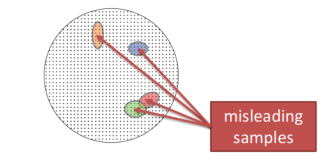
\includegraphics[scale=1.5]{images/misleading_samples.pdf}
\caption{Each point in the large circle represents a possible m-tuple of instances. Each colored oval represents the set of “misleading” m-tuple of instances for some “bad” predictor $h\in\mcl{H}_B$. The $ERM$ can potentially overfit whenever it gets a misleading training set S. That is, for some $h\in\mcl{H}_B$ we have $L_S(h)=0$. The disequations found in the demostration of the theorem guarantee that for each individual bad hypothesis, $h\in\mcl{H}_B$, atmost $(1-\varepsilon)^m$-fraction of the training sets would be misleading. In particular, the larger $m$ is, the smaller each of these colored ovals becomes. The union bound formalizes the fact that the area representing the training sets that are misleading with respect to some $h\in\mcl{H}_B$ (that is, the training sets in M) is atmostthe sum of the areas of the colored ovals. Therefore, it is bounded by $\mcl{H}_B$ times the maximum size of a colored oval. Any sample S outside the colored ovals cannot cause the $ERM$ rule to overfit.}
\end{figure}



\chapter{PAC Learning}

The title of this chapter stands for \textit{Probably Approximately Correct} learning: since the data are sampled accordingly to $\mcl{D}$, and since we can't find the perfect machine learning algorithm:
\begin{itemize} 
\item we can only be approximately correct (accuracy parameter $\varepsilon$: we are satisfied with a good $h_S$ for which $L_{\mcl{D},f}(h_S)\leq\varepsilon$)
\item we can only be probably correct (we want $h_S$ to be a good hypothesis with probability $\geq 1-\delta$)
\end{itemize}

\begin{definition}
(\textbf{PAC learnability})\\
A hypothesis class $\mcl{H}$ is PAC learnable if there exist a function $m_\mcl{H}:(0,1)^2\to\mathds{N}$ and a learning algorithm such that for every $\delta,\varepsilon\in(0,1)$, for every distribution $\mcl{D}$ over $\mcl{X}$, and for every labeling function $f:\mcl{X}\to\left\{0,1\right\}$, if the realizability assumption holds with respect to $\mcl{H},\mcl{D},f$, then when running the learning algorithm on $m\geq m_\mcl{H}(\varepsilon,\delta)$ i.i.d. examples generated by $\mcl{D}$ and labeled by $f$, the algorithm returns a hypothesis $h$ such that, with probability $\geq 1-\delta$ (over the choice of examples): $\ell_{\mcl{D},f}(h)\leq\varepsilon$.
\label{def:PAC_learn}
\end{definition}

Note: $m_\mcl{H}:(0,1)^2\to\mathds{N}$ is the sample complexity of learning $\mcl{H}$, in particular is the minimal integer that satisfies the requirements. This means that if we have an infinite number of possible hypotesis we cannot apply the theorem, but, at the same time, we can't be sure that the set is not learnable.\\

\begin{corollary}
Every finite (sufficient condition, not necessary, as said before) hypothesis class is PAC learnable with sample complexity
\[ m_\mcl{H}(\varepsilon,\delta)\leq\left[ \frac{\log(\abs{\mcl{H}}/\delta)}{\varepsilon} \right] \]
\end{corollary}

The definition of PAC learnability contains two approximation parameters. The accuracy parameter $\varepsilon$
 determines how far the output classifier can be from the optimal one and a confidence parameter $\delta$ indicating how likely the classifier is tomeet that accuracy requirement.\\

\vspace{0.5cm}
Now we would like to generalize this model, and we can do it dropping some assumptions we have made before:
\begin{itemize}
\item We remove the realizability assumption: it was interesting from a theorical point of view but too strong in many real world applications. Rejecting this means that there exist $h^*\in\mcl{H}$ such that $L_{\mcl{D},f}(h)=0$.
\item In many application it is not too realistic that the labeling is fully determined by the features we measure; for this reason it is convenient to replace the function $f$ with something more flexible, for example assuming that $\mcl{D}$ is a probability distribution over $\mcl{X}\times\mcl{Y}$ (i.e. the joint distribution over domain points and labels). One can view such a distribution as being composed of two parts: a distribution $\mcl{D}_x$ over unlabeled domain points (\textit{marginal distribution}) and a \textit{conditional} probability over labels for each domain point $D((x,y)|x)$.
\end{itemize}

\section{The empirical and the true error}
For a probability distribution $\mcl{D}$ over $\mcl{X}\times\mcl{Y}$ we redefine the true error (or risk) of a prediction rule $h$ to be
\begin{equation}
L_\mcl{D}(h) = \mathds{P}_{(x,y)\sim\mcl{D}}[h(x)\neq y] = \mcl{D}([(x,y):h(x)\neq y])
\label{eq:true_err_D}
\end{equation}

Note: in the previous definition \ref{eq:err_pred_rule} the request was $[h(x)\neq f(x)]$ but, as we said before, the function $f(x)$ doesn't exist anymore because it was a too strong assumption asking that the labels were fully determined by a single function.\\
The definition of the empirical risk, instead, remains the same as before
\[ L_S(h)=\frac{[i\in[m]:h(x_i)\neq y_i]}{m} \]
and still represent the probability that, for a pair $(x_i,y_i)$ taken uniformily at random training data, the event "$h(x_i)\neq y_i$" holds.

\section{The Bayes optimal predictor}
Given any probability distribution $\mcl{D}$ over $\mcl{X}\times [0,1]$, the best label predicting function (the one that minimize $L_\mcl{D}(h)$) will be
\begin{equation}
f_\mcl{D}(x) = \left\{\begin{aligned} &1\quad \text{if  } \mathds{P}[y=1|x]\geq 1/2\\ &0\quad \text{otherwise}\end{aligned}\right.
\label{eq:bayes_predictor}
\end{equation}

It's easy to verify that the predictor $f_\mcl{D}$ is optimal, in the sense that any other classifier $g:\mcl{X}\to [0,1]$, has a lower error, $L_\mcl{D}(f_\mcl{D})\leq L_\mcl{D}(g)$.\\
This optimal predictor is interensting from a theorical point of view, but unfortunately is not usable in practice because e don't know the distribution $\mcl{D}$ and, consequently $\mathds{P}[y=1|x]$.\\


\section{Agnostic PAC Learnability}
Clearly, we cannot hope that the learning algorithm will find a hypothesis whose error is smaller than the minimal possible error, that of the Bayes predictor. Furthermore, as we shall prove later, once we make no prior assumptions about the data-generating distribution, no algorithm can be guaranteed to find a predictor that is as good as the Bayes optimal one. Instead, we require that the learning algorithm will find a predictor whose error is not much larger than the best possible error of a predictor in some given benchmark hypothesis class. Of course, the strength of such a requirement depends on the choice of that hypothesis class.\\
\begin{definition}(\textbf{Agnostic PAC Learnability})\\
A hypothesis class $\mcl{H}$ is agnostic PAC learnable if there exist a function $m_\mcl{H}:(0,1)^2\to\mathds{N}$ and a learning algorithm such that for every $\delta,\varepsilon\in (0,1)$ and for every distribution $\mcl{D}$ over $\mcl{X}\times\mcl{Y}$, when running the algorithm on $m\geq m_\mcl{H}(\varepsilon,\delta)$ i.i.d. examples generated by $\mcl{D}$ the algorithm returns a hypothesis $h$ such that, with probability $\geq 1-\delta$ (over the choice of the $m$ training examples):
\[ L_\mcl{D}(h)\leq\min_{h'\in\mcl{H}}L_\mcl{D}(h')+\varepsilon \]
\label{def:agnostic_PAC_l}
\end{definition}
Notes on the definition:
\begin{itemize}
\item The agnostic PAC learning generalizes the definition of PAC learning, in the sense that, if the realizability assumption holds, this new definition provides the same guarantee as the previous one.
\item The realizability assumption would implies that the quantity $\min_{h'\in\mcl{H}}L_\mcl{D}(h')$, that represents the performance of the best possible classifier (for example the Bayes' one), is always equal to zero.
\end{itemize}
Anyway a learner can still declare success if its error is not much larger than the best error achievable by a predictor from the class $\mcl{H}$. This is in contrast to PAC learning, in which the learner is required to achieve a small error in absolute terms and not relative to the best error achievable by the hypothesis class.\\ 

\vspace{0.5cm}
We now want to extend our model so that it can be applied to a wide variety of learning tasks. Let's consider 3 different possible problems:
\begin{itemize}
\item \textit{Binary and Multiclass classification}: our training sample will be a finite sequence of (feature vector,label) pairs, the learner’s output will be a function from the domain set to the label set, and, finally, for our measure of success, we can use the probability, over pairs, of the event that our predictor suggests a wrong label.
\item \textit{Regression}: in this task, one wishes to find some simple pattern in the data, a function between $\mcl{X}$ and $\mcl{Y}=\mathds{R}$. For the loss function, we can't use the same of the previous case, we need a new one.
\end{itemize}

\subsection{Generalized loss function}
Given any set $\mcl{H}$ (that plays the role of our hypotheses, or models) and some domain $Z$ let $\ell$ be any function from $\mcl{H}\times Z$ to the set of nonnegative real numbers, $\ell:\mcl{H}\times Z\to\mathds{R}+$. We call such functions loss functions.\\
We now define the \textbf{risk function} to be the expected loss of a classifier $h\in\mcl{H}$, with respect to a probability distribution $\mcl{D}$ over $Z$, namely:
\begin{equation}
L_\mcl{D}(h) = \mathds{E}_{z\sim\mcl{D}}\left[\ell(h,z)\right]
\label{eq:risk_func}
\end{equation}
Similarly, we define the \textbf{empirical risk} to be the expected loss over a given sample $S=(z_1,\dots,z_m)\in Z^m$, namely:
\begin{equation}
L_S(h) = \frac{1}{m}\sum_{i=1}^m\ell(h,z_i)
\label{eq:emp_risk}
\end{equation}

We must keep in mind that the loss always depends on the problem, there isn't a universal one. Sometimes it is useful to create a "personalized" loss function.\\
Common loss functions:
\begin{itemize}
\item \textit{0-1 loss}: commonly use in binary or multiclass classification (obviously is not the only possible solution, is just the simpler and most common one).
\[ \ell_{0-1}(h,(x,y))=\left\{\begin{aligned} &0\quad\text{if  }h(x)=y\\ &1\quad\text{if  }h(x)\neq y\end{aligned}\right. \]
\item \textit{Squared loss L2}: commonly used in regression, penalize few large errors.
\[ \ell_{sq}(h,(x,y))=(h(x)-y)^2 \]
\item \textit{Absolute value loss L1}: commonly used in regression, penalize many small errors:
\[ \ell_{abs}(h,(x,y))=\abs{h(x)-y} \]
\end{itemize}

\begin{example} The loss function depends on our problem!
Let's image a machine learning algorithm that verify fingerprints to guarantee the access to something. There are essentially two types of error that the computer can do:
\begin{itemize}
\item \textit{False accept}: when accepts an unauthorized user.
\item \textit{False reject}: when doesn't accept an athorized user.
\end{itemize}
If, for example, a supermarket implement the algorithm to give discounts:
\begin{itemize}
\item[-] False reject is costly; just the customer gets annoyed.
\item[-] False accept is minor, the supermarket lose just a discount and the intruder left his fingerprints.
\end{itemize}
If, instead, a similar algorithm has been implemented by CIA for the security of a certain area:
\begin{itemize}
\item[-] False reject can be tolerade.
\item[-] False accept is a disaster!
\end{itemize}
This example want to show that often the loss function need to be "calibrated" by our knowledge on the problem, to understand which errors are tolerable and which are not.
\end{example}

\begin{definition} (\textbf{Agnostic PAC Learnability for General Loss 
Functions})\\
Recalling the definition \ref{def:agnostic_PAC_l}, for which the hypothesis generate by the algorithm (with probability $\geq 1-\delta$ over the training set) has a true error
\[ L_\mcl{D}(h)\leq\min_{h'\in\mcl{H}}L_\mcl{D}(h')+\varepsilon \]
we can implement the definition we have written for the loss function deducing that:
\[ L_\mcl{D}(h) = \mathds{E}_{z\sim\mcl{D}}\left[\ell(h,z)\right] \]
\label{def:agnosticPAC_general_loss}
\end{definition}


\chapter{Learning from Uniform Convergence}

Recall that, given a hypothesis class $\mcl{H}$, the ERM learning paradigm works as follow: upon receiving a training sample S, the learner evaluates the error of each $h\in\mcl{H}$ on the given sample and outputs a member of the class that minimizes this empirical risk. The hope is that an $h$ that minimizes the empirical risk with respect to S is a risk minimizer with respect to the true data probability distribution aswell. For this reason we want that the empirical error is a good approximation of the true error for all the solutions, and not only for the best one ($L_S(h)$ is similar to $L_\mcl{D}(h)$, $\forall\, h$).\\
\begin{definition} (\bm{$\varepsilon$}\textbf{-representative})\\
A training set S is called $\varepsilon$-representative (with respect to domain Z, hypothesis class $\mcl{H}$, loss function $\ell$ and distribution $\mcl{D}$) if 
\[ \forall h\in\mcl{H} \quad \abs{L_S(h)-L_D(h)}\leq\varepsilon \]
\end{definition}  

This is a stronger request than previous ones because we do not more focus on the best hypothesis of the class.\\

\begin{theorem}
	Assume that the training set $S$ is $\frac{\varepsilon}{2}$-representative. Then, any output of $ERM_\mcl{H}(S)$ (i.e. any $h_S\,\in\,\underset{h\in\mcl{H}}{argmin}\, L_S(h)$) satisfies:
	\[ L_\mcl{D}(h_S)\leq\min_{h\in\mcl{H}} L_\mcl{D}(h)+\varepsilon  \]
\end{theorem} 
\begin{proof}
	For every $h\in\mcl{H},$
	\[ L_\mcl{D}(h_S)\leq L_S(h_S)+\frac{\varepsilon}{2}\leq L_\mcl{D}(h)+\frac{\varepsilon}{2}+\frac{\varepsilon}{2} = L_\mcl{D}(h) + \varepsilon\]
	where the first and the third inequalities are due to the assumption that $S$ is $\frac{\varepsilon}{2}$- and the second inequality holds since $h_S$ is an ERM predictor. 
\end{proof}

The relation guarantee by the theorem is exactly the one required by the definition of agnostic PAC learnability: in fact, the consequence of this statement is that if, with probability at least $1-\delta$, a random training set $S$ is $\varepsilon$-representative, then the ERM rule is an agnostic PAC learner.

\begin{definition} (\textbf{Uniform Convergence})\\
	A hypothesis class $\mcl{H}$ has the uniform (same $m$ for all $h$ and all $\mcl{D}$) convergence property (with respect to a domain $Z$ and a loss function $\ell$) if there exists a function $m_\mcl{H}^{UC}:(0,1)^2\to\mathds{N}$ such that for every $\varepsilon,\delta\in(0,1)$ and for every probability distribution $\mcl{D}$ over $Z$, if $S$ is a sample of $m\geq m_\mcl{H}^{UC}(\varepsilon,\delta)$ i.i.d. examples drawn from $\mcl{D}$, then with probability $\geq 1-\delta$, $S$ is $\varepsilon$-representative.
\end{definition} 

This means that the function $m_\mcl{H}^{UC}$ measures the (minimal) sample complexity of obtaining the uniform convergence property, namely, how many examples we need to ensure that with probability at least $1-\delta$ the sample would be $\varepsilon$-representative.

\begin{proposition}
	If a class $\mcl{H}$ has the uniform convergence property with a function $m_\mcl{H}^{UC}$ then the class is agnostically PAC learnable with the sample complexity $m_\mcl{H}(\varepsilon,\delta)\leq m_\mcl{H}^{UC}(\varepsilon/2,\delta)$. Furthermore, in that case the $ERM_\mcl{H}$ paradigm is a successful agnostic PAC learner for $\mcl{H}$.	
\end{proposition}

\begin{proposition}
	Let $\mcl{H}$ be a finite hypothesis class, let $Z$ be a domain, and let $\ell:\mcl{H}\times Z\to[0,1]$ be a loss function. Then:
	\begin{itemize}
		\item $\mcl{H}$ enjoys the uniform convergence property with sample complexity 
		\[ m_\mcl{H}^{UC}(\varepsilon,\delta)\leq\left[\frac{\log(2\abs{\mcl{H}}/\delta)}{2\varepsilon^2}\right] \]
	\item $\mcl{H}$ is agnostically PAC learnable using the ERM algorithm with sample complexity
	\[ m_\mcl{H}(\varepsilon,\delta)\leq m_\mcl{H}^{UC}(\varepsilon/2,\delta)\leq\left[\frac{2\log(2\abs{\mcl{H}}/\delta)}{\varepsilon^2}\right] \]
	\end{itemize}
\end{proposition}
\begin{proof}
	Fix some $\varepsilon,\delta$. We need to find a sample size $m$ that 
	guarantes that for any $\mcl{D}$, with probability at least $1-\delta$ of 
	the choice of $S=(z_1,\dots,z_m)$ sampled i.i.d. from $\mcl{D}$ we have 
	that for all $h\in\mcl{H}$, $\abs{L_S(h)-L_\mcl{D}(h)}\leq\varepsilon$ (so 
	we are asking $S$ to be $\varepsilon$-representative for some $m$). Namely
	\[ \mcl{D}^m\left(\left\{S:\forall 
	h\in\mcl{H},\abs{L_S(h)-L_\mcl{D}(h)}\leq\varepsilon \right\}\right)\geq 
	1-\delta \]	 
	Equivalently, we need to show that the probability of \textit{not} having 
	uniform convergence is
	\[ \mcl{D}^m\left(\left\{S:\exists h\in\mcl{H},\abs{L_S(h)-L_\mcl{D}(h)} > 
	\varepsilon \right\}\right)\leq \delta \]	
	In the expression above, I can rewrite the set as the union over $h$:
	\[ \left\{S:\exists h\in\mcl{H},\abs{L_S(h)-L_\mcl{D}(h)} > 
	\varepsilon \right\} = 
	\bigcup_{h\in\mcl{H}}\left\{S:\abs{L_S(h)-L_\mcl{D}(h)} > 
	\varepsilon \right\} \] 
	and, applying the Union Bound (\ref{eq:union_bound}), we obtain
	\[ \mcl{D}^m\left(\left\{S:\exists h\in\mcl{H},\abs{L_S(h)-L_\mcl{D}(h)} > 
	\varepsilon 
	\right\}\right)\leq\sum_{h\in\mcl{H}}\mcl{D}^m\left\{S:\abs{L_S(h)-L_\mcl{D}(h)}
	 > \varepsilon \right\} \]
	 The next step will be to show that for any fixed hypothesis $h$, the gap 
	 between the true and the empirical risk is likely to be small (for a 
	 sufficiently large $m$).\\
	 Now, recall that 
	 $L_\mcl{D}(h)=\mathds{E}_{z\sim\mcl{D}}\left[\ell(h,z)\right]$ 
	 (\ref{def:agnosticPAC_general_loss}) and that 
	 $L_S(h)=\frac{1}{m}\sum_{i=1}^m\ell(h,z_i)$ (\ref{eq:emp_risk}). Since 
	 each $z_i$ is sampled i.i.d. from $\mcl{D}$, the expected value of the 
	 random variable $\ell(h,z_i)$ is $L_\mcl{D}(h)$. By the linearity of 
	 expectation, it follows that $L_\mcl{D}(h)$ is also the expected value of 
	 $L_S(h)$. Hence, the quantity $\abs{L_S(h)-L_\mcl{D}}$ is the deviation of 
	 the random variable $L_S(h)$ from its expectation. A basic statistical 
	 fact, the law of large numbers, states that when $m$ goes to infinity, 
	 empirical averages converge to their true expectation, and this is also 
	 valid for $L_S(h)$, since it is the empirical average of $m$ i.i.d. 
	 samples.\\
	 However, this low is only an asymptotic result, and it provides no 
	 information about the gap between empirical averages and their expected 
	 value: to quantify this gap we will use a measure concentration inequality 
	 due to Hoeffding:
	 \begin{lemma}
	 	(\textbf{Hoeffding's Inequality})\\
	 	Let $\theta_1,dots,\theta_m$ be a sequence of i.i.d. random variables 
	 	and assume that for all $i$, $\mathds{E}[\theta_i]=\mu$ and 
	 	$\mathds{P}[a\leq\theta_i\leq b]=1$. Then, for any $\varepsilon>0$:
	 	\[ \mathds{P}\left[\abs{\frac{1}{m}\sum_{i=1}^m 
	 	\theta_i-\mu}>\varepsilon\right]\leq 
	 	2\exp(-\frac{2m\varepsilon^2}{(b-a)^2}) \]\\
	 	\label{lem:Hoeffding}
	 \end{lemma}
 Getting back to our problem, let $\theta_i$ be the random variable 
 $\ell(h,z_i)$. Since $h$ is fixed and $z_1,\dots,z_m$ are sample i.i.d., it 
 follows that $\theta_1,\dots,\theta_m$ are also i.i.d. random variables. 
 Furthermore, $L_S(h)=\frac{1}{m}\sum_{i=1}^m\theta_i$ and $L_\mcl{D}(h)=\mu$. 
 Let us further assume that the range of $\ell$ is $[0,1]$. We therefore obtain 
 that
 \[ \mcl{D}^m\left\{S:\abs{L_S(h)-L_\mcl{D}(h)} > \varepsilon \right\} = 
 \mathds{P}\left[\abs{\frac{1}{m}\sum_{i=1}^m \theta_i-\mu}>\varepsilon\right] 
 \leq 2\exp(-2m\varepsilon^2) \]
 Applying this to the sum over $h$:
 \[ \sum_{h\in\mcl{H}}\mcl{D}^m\left\{S:\abs{L_S(h)-L_\mcl{D}(h)} > \varepsilon 
 \right\} \leq\abs{\mcl{H}}2e^{-2m\varepsilon^2} \]
 Now, we need to find $m$ for which the term on the right above is smaller or 
 equal than $\delta$, so we fix
 \[ m\geq \frac{\log(2\abs{\mcl{H}}/\delta)}{2\varepsilon^2} \]
 So that
 \[ \mcl{D}^m\left\{S:\abs{L_S(h)-L_\mcl{D}(h)} > \varepsilon \right\} 
 \leq\delta \]
\end{proof}

\subsection{The Discretization Trick}
While the previous theorem only applies on finite hypothesis classes, there is a simple trick that allow us to get a very good estimate of the practical sample complexity of infinite hypothesis classes. In many real world application, in fact, we consider classes determined by a set of parameters in $\mathds{R}$.\\
The solution arises when we use computers. Using a pc, in fact, we will probably maintain real numbers using floating point representation, say, of 64 bits. It follows that, in practice, our hypothesis class is parameterized by the set of scalar that can be represented using a 64 bits floating point number. There are at most $2^{64}$ such numbers; hence the actual size of our hypothesis class is at most $2^{64}$. More generally, if our hypothesis class is parameterized by $d$ numbers, in practice we learn an hypothesis class of size at most $2^{64d}$.\\
Applying the proposition, we obtain that the sample complexity of such classes is bounded by
\[ m_\mcl{H}(\varepsilon,\delta)\leq m_\mcl{H}^{UC}(\varepsilon/2,\delta)\leq \frac{2\log\left(2\frac{2^{64d}}{\delta}\right)}{\varepsilon^2} \] 
This upper bound on the sample complexity has the deficiency of being dependent on the specific representation of real numbers used by our machine.


\chapter{The Bias-Complexity Trade-Off}
In one of the previous chapters we saw that, unless one is careful, the training data can mislead the learner, and result in overfitting. To overcome this problem, we restricted the search space to some hypothesis class $\mcl{H}$. Such an hypothesis class can be viewed as reflecting some prior knowledge that the learner has about the task – a belief that one of the members of the class $\mcl{H}$ is a low-error model for the task.\\
Our main objective was, given a training set $S$ and a loss function, to find a function $\hat{h}$ for which the error $L_\mcl{D}(\hat{h})$ is small (that brought to the definition of Agnostic PAC learnability (\ref{def:agnostic_PAC_l})). For this reason we needed a large hypothesis class to contain the best solution, but at the same time a good algorithm to find it.\\
But, is there some kind of universal learner, that is, a learner who has no prior knowledge about a certain task and is ready to be challenged by any task, that predicts the best $\hat{h}$ for any distribution $\mcl{D}$?\\
So, what about using the set of \textit{all} the functions from $\mcl{X}$ to $\mcl{Y}$ as the hypothesis class? With this assumption we would be sure that the solution (if the problem is solvable) is inside the class.\\

\begin{theorem} (\textbf{No-Free Lunch})\\
	Let $A$ be a learning algorithm for the task of binary classification with respect to the 0-1 loss over a domain $\mcl{X}$. Let $m$ be any number smaller than $\abs{\mcl{X}}/2$, representing a training set size. Then, there exists a distribution $\mcl{D}$ over $\mcl{X}\times\left\{0,1\right\}$ such that:
	\begin{itemize}
		\item there exists a function $f:\mcl{X}\to\left\{0,1\right\}$ with $L_\mcl{D}(f)=0$ (so a perfect solution with 0 loss)
		\item with probability of at least $1/7$ over the choice $S\sim\mcl{D}^m$ we have that $L_\mcl{D}(A(S))\geq 1/8$.
	\end{itemize}
\end{theorem} 
This means that there isn't a universal learner: the algorithm can fail even if there is a perfect solution for the training set. In fact, the theorem guarantees the existance of this perfect solution (with 0 loss), but doesn't guarantee a good performance instead.\\
The key message is that for every ML algorithm there exist a task on which it fails even if another ML algorithm is able to solve it.\\

\vspace{0.3cm}
\textit{Idea of the proof}: our training set is smaller than half of the domain. This means that we have no information on what happens on the other half, but we can suppose that there is some target function f that works on the other half in a way that contradicts our estimated labels.\\

\vspace{0.5cm}
Let's consider an ERM predictor over the hypothesis class of all the functions $f:\mcl{X}\to\left\{0,1\right\}$. This class represent a lack of knowledge: every possible function is considered a good candidate. According to the previous theorem, any algorithm that chooses its output from an hypothesis belonging to that class, and in particular the ERM predictor, will fail on some learning task. Therefore, the class is not PAC learnable, as formalized in the following corollary.\\
\begin{corollary}
	Let $\mcl{X}$ be an infinite domain set and let $\mcl{H}$ be the set of all the functions from $\mcl{X}$ to $\left\{0,1\right\}$. Then, $\mcl{H}$ is not PAC learnable.
\end{corollary}

\begin{proof}
	Let's assume, by way of contradiction, that the class is learnable and let's choose some $\varepsilon <1/8$ and $\delta <1/7$. By the definition of PAC learnability (\ref{def:PAC_learn}), it exists an algorithm $A$ and an integer $m=m(\varepsilon,\delta)$, such that for any data-generating distribution over $\mcl{X}\times\left\{0,1\right\}$, if for some function $f$ in that domain, $L_\mcl{D}(f)=0$, then with probability $\geq 1-\delta$ when $A$ is applied to samples $S$ of size $m$, generated i.i.d. by $\mcl{D}$, $L_\mcl{D}(A(S))\leq\varepsilon$.\\
	However, applying the Free-Lunch theorem, since $\abs{\mcl{X}}>2m$, for every learning algorithm (and in particular for $A$), there exists a distribution $\mcl{D}$ such that with probability greater than $1/7 >\delta$, $L_\mcl{D}(A(S)) >1/8 >\varepsilon$, which leads to the desired contradiction.
\end{proof}

But how can we prevent such failures? We should, for example, use our knowledge on a specific learning task to avoid distributions that will cause us to fail.\\
But how should we choose a good hypothesis class? On the other hand we want to believe that this class includes the hypothesis that has no error at all (in the PAC setting), or at least that the smallest error achievable by a hypothesis from this class is indeed rather small (in the agnostic setting). On the other hand, we have just seen that we cannot simply choose the richest class i.e. the class of all functions over the given domain.\\
\begin{itemize}
	\item If we choose a \textit{small} $\mcl{H}$ we will deal with \textit{low approximation capabilities} (large $L_S$) but \textit{good generalization properties} ($L_\mcl{D}\sim L_S$). So the approximation found will work similarly on real data as on the training set, but it's not guarantee that the best hypothesis is in the class.
	\item If we choose a \textit{large} $\mcl{H}$, instead, we will have \textit{good approximation capabilities} (small $L_S$) but there is a bigger \textit{risk of overfitting} ($L_\mcl{D}\gg L_S$). Moreover the no free lunch theorem suggests to not have too larger hypothesis classes.
\end{itemize}

\section{Error Decomposition}
\label{sec:err_dec}
To answer these questions we decompose the true error of an $ERM_\mcl{H}$ predictor, $h_S$ into two components, as follows:
\[ L_\mcl{D}(h_S)=\varepsilon_{app}+\varepsilon_{est} \]

\begin{itemize}
	\item \textbf{Approximation error}
	\[ \varepsilon_{app}=\min_{h\in\mcl{H}} L_\mcl{D}(h) \]
	It is the minimum risk achievable by a predictor in the hypothesis class. It does not depend on the training set, or on the sample size, but only on the choice of the class. Enlarging the hypothesis class can decrease the approximation error. Under the realizability assumption, this error is zero.
	\item \textbf{Estimation error}
	\[ \varepsilon_{est} = L_\mcl{D}(h_S) - \min_{h\in\mcl{H}}(h) \]
	It is the difference between the approximation error and the error achieved by the ERM predictor. The estimation error results because the training error is only an estimate of the true risk, and so the predictor minimizing the empirical risk is only an estimate of the predictor minimizing the true risk. This type of error depends on the training set size and on the size, or complexity, of the hypothesis class. For a finite class, the estimation error increases (logarithmically) with $\abs{\mcl{H}}$ and decreases with $m$ (so the training error becomes a good estimate of the true error).
\end{itemize}

The following pictures schematized what we just said regarding the two types of error.

\begin{figure}[!h]
	\centering
	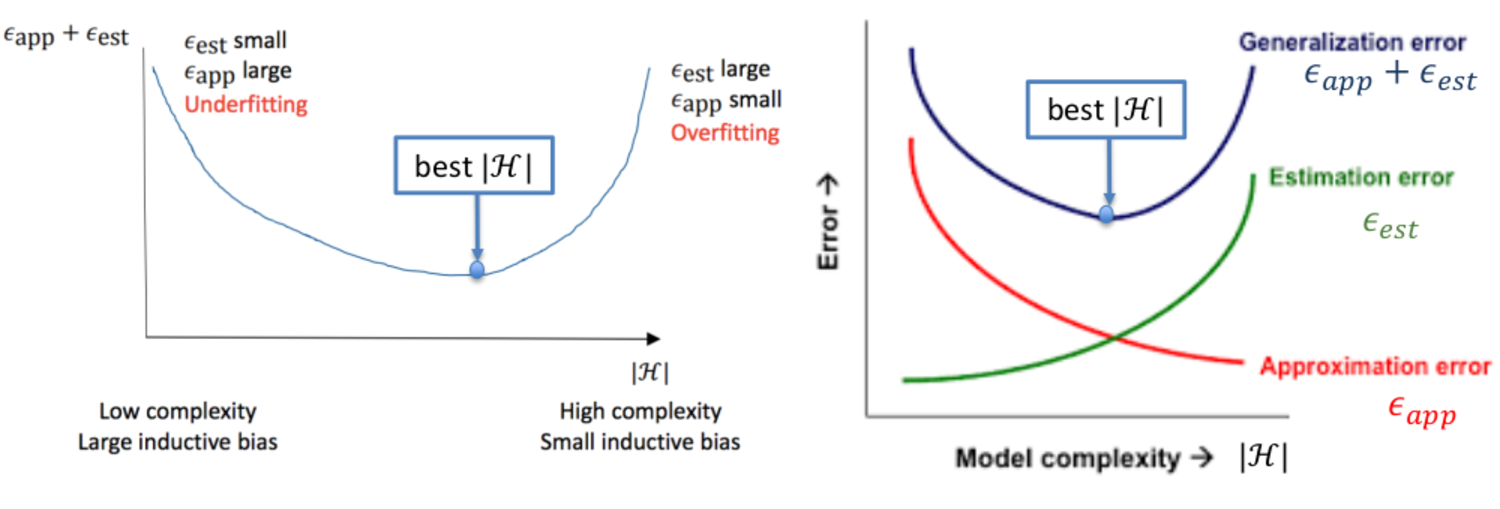
\includegraphics[scale=0.5]{images/error_decomposition.pdf}
	\caption{Error decomposition}
	\label{fig:err_dec}
\end{figure}

Since our goal is to minimize the total risk, we face a \textit{tradeoff}, called the \textbf{bias complexity tradeoff}. On one hand, choosing $\mcl{H}$ to be a very rich class decreases the approximation error but at the same time might increase the estimation error, as a rich $\mcl{H}$ might lead to \textit{overfitting}. On the other hand, choosing $\mcl{H}$ to be a very small set reduces the estimation error but might increase the approximation error or, in other words, might lead to \textit{underfitting}.\\
The differences between overfitting and underfitting can be seen in picture \ref{fig:under_over_fit}.\\

\begin{figure}[!h]
	\centering
	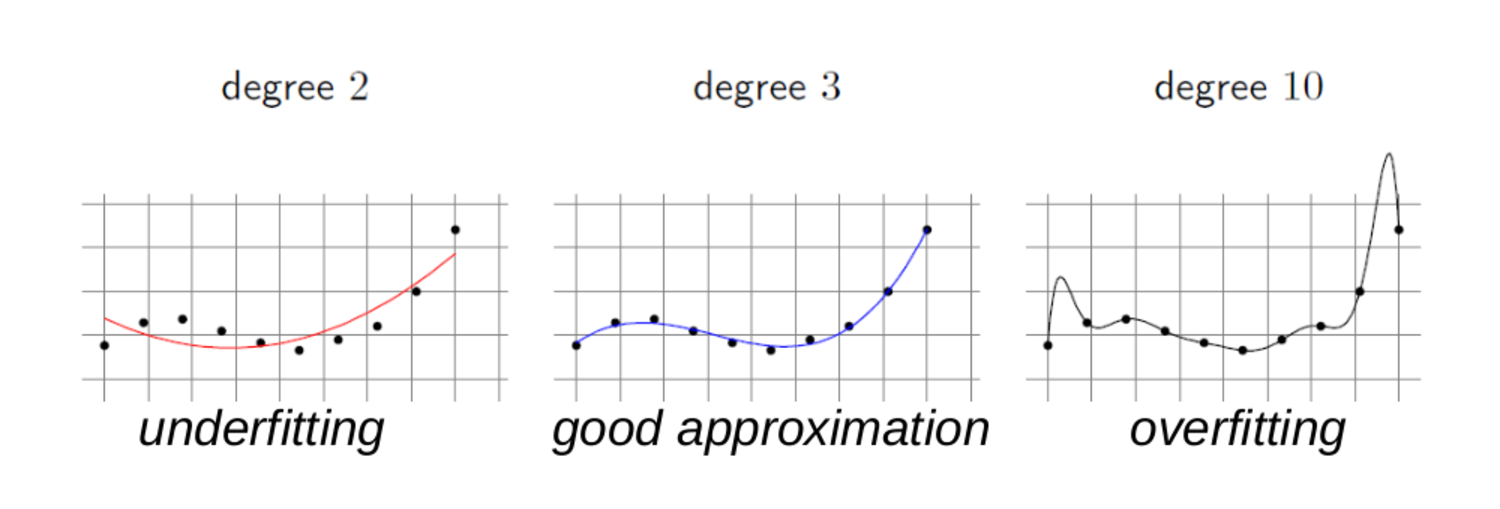
\includegraphics[scale=0.7]{images/over_under_fitting.pdf}
	\caption{Comparison between underfitting and overtitting}
	\label{fig:under_over_fit}
\end{figure}

\vspace{0.5cm}
We need to estimate the generalization error $L_\mcl{D}(h)$ for a function h (the one selected with ERM). To do this, we use a \textit{test set}, a new set of samples different (disjoint) from the training set used to pick h. Sometimes we use also a \textit{validation set} for selecting the hyper-parameters of the algorithm or to evaluate errors while iterative training procedures are running.\\
To summarize the procedure of training a ML algorithm parametrized by some Hyper-Parameters (HP):
\begin{itemize}
	\item[1.] Select Hyper-Parameters values
	\item[2.] Train the algorithm with the choosen parameters on the training set
	\item[3.] Evaluate performances on the validation set
	\item[4.] Go back to 1. and select new HP values
	\item[5.] Select the final HP leading to the smallest validation error
	\item[6.] Compute error estimation on the test set  
\end{itemize}


\chapter{Linear Predictors}
In this chapter we will study the family of linear predictors, one of the most 
useful families of hypothesis classes. Many learning algorithms widely used in 
practice, rely on linear predictors, because of their intuitiveness and ease of 
interpretation, as well as for their efficiency.\\
We will introduce several hypothesis classes:
\begin{itemize}
	\item Halfspaces (classification)
	\item Linear Regression (regression)
	\item Logistic Regression (classification modeled as a regression problem)
\end{itemize}
and the algorithms to find the predictors:
\begin{itemize}
	\item Linear Programming (for halfspaces)
	\item Perceptron (for halfspaces)
	\item Least Squares (for regression)
\end{itemize}
  
First, we define the class of affine functions:
\[ L_d=\left\{h_{\vb{w},b}:\vb{w}\in\mathds{R}^d,b\in\mathds{R} \right\} \]
where
\[ h_{\vb{w},b}(\vb{x})= \sprod{w}{x}+b = \left(\sum_{i=1}^d w_ix_i\right)+b \]
Each member of $L_d$ is a function $\vb{x}\to\sprod{w}{x}+b$ parameterized by a 
vector $\vb{w}\in\mathds{R}^d$ (of \textit{weights}) and a scalar (called 
\textit{bias}) $b\in\mathds{R}$.\\
The different hypothesis classes of linear predictors are composition of functions $\phi:\mathds{R}\to\mcl{Y}$ on $L_d$. For example, in binary classification, we can choose $\phi$ to be the sign function, and for regression problems, where $\mcl{Y}=\mathds{R}$, $\phi$ is simply the identity function.\\
We can give a (2D) geometric interpretation of this functions. As can be seen in figure \ref{fig:affine_geom}:
\begin{figure}[!h]
	\centering
	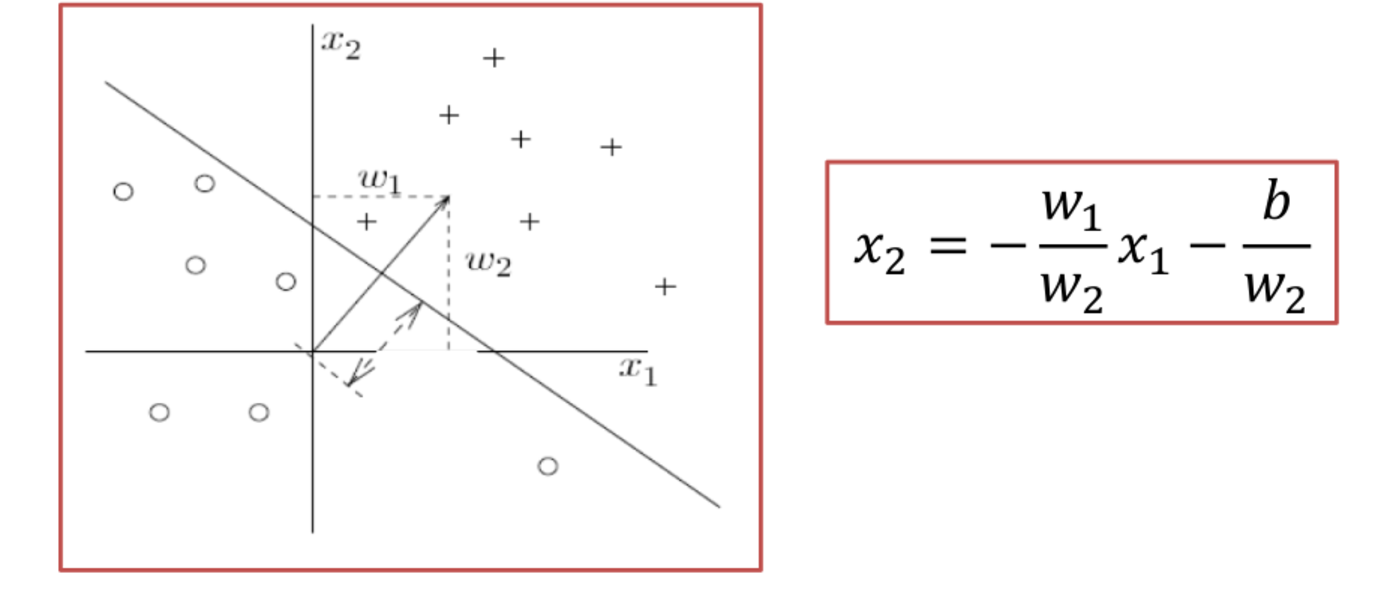
\includegraphics[scale=0.5]{images/affine_geometry.pdf}
	\caption{Geometrical interpretation of the class of affine functions}
	\label{fig:affine_geom}
\end{figure}
\begin{itemize}
	\item The bias is proportional to the offset of the line from the origin
	\item The weights determine the slope of the line
	\item The weight vector is perpendicular to the line
\end{itemize} 
It may be more convenient to incorporate the bias $b$ into the vector $\vb{w}$ 
as an extra coordinate with a value of 1 in all $x\in\mcl{X}$; namely let 
$\vb{w}'=(b,w_1,\dots,w_d)\in\mathds{R}^{d+1}$ and let 
$\vb{x}'=(1,x_1,\dots,x_d)\in\mathds{R}^{d+1}$. Therefore:
\[ h_{\vb{w},b}(\vb{x})=\sprod{w}{x}+b=\sprod{w'}{x'} \]
It follows that each affine function in $\mathds{R}^d$ can be rewritten as an 
\textit{homogeneous} linear function in $\mathds{R}^{d+1}$ applied over the 
transformation that appends the constant 1 to each input vector. Therefore, 
whenever it simplifies the presentation, we will omit the bias term and refer 
to $L_d$ as the class of homogeneous linear functions of the form 
$h_{\vb{w}}(\vb{x})=\sprod{w}{x}$.

\section{Halfspaces}
The first hypothesis class we consider is the class of halfspaces, designed for 
binary classification problems, namely $\mcl{X}=\mathds{R}^d$ and 
$\mcl{Y}=\left\{-1,1\right\}$. The class of halfspaces is defined as follow:
\[ HS_d=sign\circ L_d \left\{\vb{x}\to 
sign\left(h_{\vb{w},b}(\vb{x})\right):h_{\vb{w},b}\in L_d \right\} \]
In other words, each halfspace hypothesis in $HS_d$ is parameterized by 
$\vb{w}\in\mathds{R}^d$ and $b\in\mathds{R}$ and upon receiving a vector 
$\vb{x}$ the hypothesis returns the label 
$sign\left(\sprod{\vb{w}}{\vb{x}}+b\right)$.\\
To illustrate this hypothesis class geometrically, it is instructive to 
consider the case $d=2$.
\begin{figure}[!h]
	\centering
	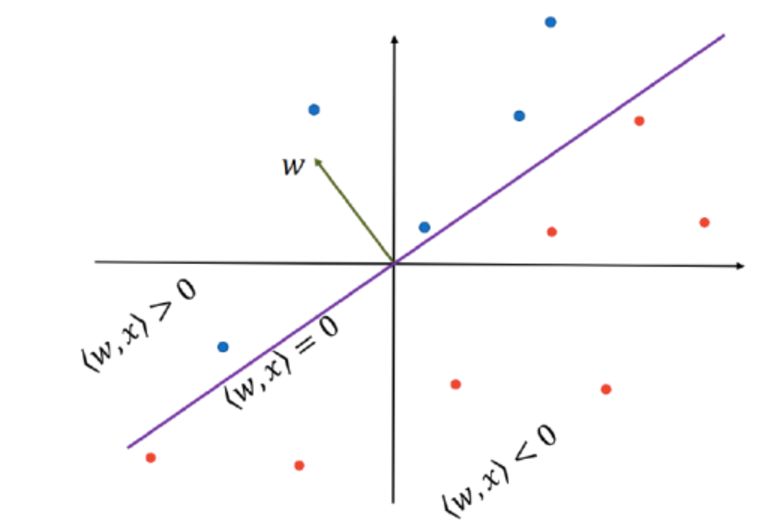
\includegraphics[scale=0.5]{images/halfspaces_2D.pdf}
	\caption{Two-dimensional representation of halfspaces}
	\label{fig:halfspaces_2D}
\end{figure}
Each hypothesis forms a hyperplane that is perpendicular to the vector $\vb{w}$ 
and intersects the vertical axis at the 
point $(0,-b/w_2)$. The instances that are "above" the hyperplane, that share 
an acute angle with $\vb{w}$, are labeled positively. Instances that are 
"below" the hyperplane, that share an obtuse angle with $\vb{w}$, are labeled 
negatively. An example can be seen in figure \ref{fig:halfspaces_2D}.\\
However, as we can see from figure \ref{fig:halfspaces_realizability}, to find 
an ERM halfspace we need to be in a realizable case: in this context, the 
realizable case is often referred to the \textit{separable} case, since it is 
possible to separate with an hyperplane all the positive examples from all the 
negative ones, while it is computationally hard to implement the ERM rule in 
the non separable case (agnostic case).
\begin{figure}[!h]
	\centering
	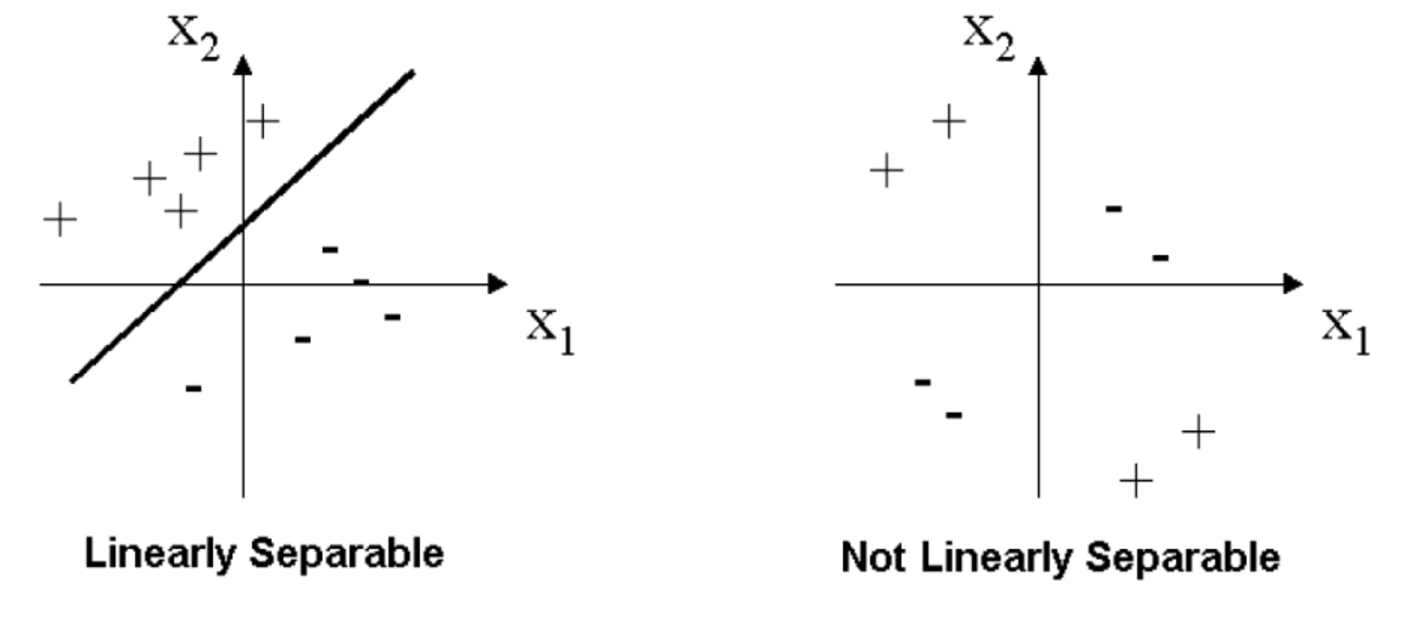
\includegraphics[scale=0.5]{images/halfspaces_realizability.pdf}
	\caption{Realizability condition of ERM algorithm for halfspaces}
	\label{fig:halfspaces_realizability}
\end{figure}

\subsection{Linear Programming for the Class of Halfspaces}
\textit{Linear programs} (LP) are problems that can be expressed as maximizing 
a linear function subject to linear inequalities. The main target, consist into 
finding the quantity $\max_{\vb{w}\in\mathds{R}^d} \sprod{u}{w}$ subject to 
$A\vb{w}\geq\vb{v}$ where $\vb{w}\in\mathds{R}^d$ is the vector of variables we 
wish to determine, $A$ is a $m\times d$ matrix and $\vb{v}\in\mathds{R}^m$ and 
$\vb{u}\in\mathds{R}^d$ are vectors. Linear programs can be solved efficiently 
namely, in a polinomial time.\\
Let's assume, for simplicity, the homogeneous case, and let 
$S=\left\{(\vb{x_i},y_i)\right\}_{i=1}^m$ be a training set of size $m$. Sinc 
we assume the realizable case, an ERM predictor should have zero errors on the 
training set ($L_S(h_S)$). So we are looking for some vector 
$\vb{w}\in\mathds{R}^d$ for which $sign\left(\sprod{w}{x_i}\right)=y_i$; or, 
equivalently, $y_i\sprod{w}{x_i}>0$ $\forall i=1,\dots,m$. Let $\vb{w^*}$ be a 
vector that satisfies this condition (it must exist since we assumed 
realizability). Define $\gamma=\min_i\left(y_i\sprod{w^*}{x_i}\right)$ and let 
$\vb{\bar{w}}=\vb{w}/\gamma$. Therefore, for all $i$ we have
\[ y_i\sprod{\bar{w}}{x_i}= \frac{1}{\gamma}y_i\sprod{w^*}{x_i}\geq 1 \]
We have thus shown that there exist a vector that satisfy  
$y_i\sprod{w}{x_i}\geq 1$ and clearly, such a vector is an ERM predictor.\\
To find a vector that satisfy the previous equation we have to use the 
following procedure: set $A$ to be the $m\times d$ matrix whose rows are the 
instances multiplied by $y_i$. Namely $A_{ij}=y_i x_{i,j}$ where $x_{i,j}$ 
represents the j-th component of the vector $\vb{x_i}$. Let $\vb{v}$ be the 
vector $(1,\dots,1)\in\mathds{R}^m$. Then, we can re-write the previous 
equation as $A\vb{w}\geq\vb{v}$.\\
This procedure requires also a maximization object, because the $\vb{w}$ that 
satisfy the constraints are equal candidates as output hypothesis. For this 
reason, we set a "dummy" objective $\vb{u}=(0,\dots,0)\in\mathds{R}^d$.

\subsection{Perceptron for Halfspaces}
A different implementation of the ERM rule is the Perceptron algorithm of 
Rosenblatt (1938). The main target of this algorithm is to find the vector 
$\vb{w}$ that represents the separating hyperplane, in homogeneous 
coordinates.\\
The Perceptron is an iterative algorithm that construct a sequence of vectors 
$\vb{w}^{(1)},\vb{w}^{(2)},\dots$, starting from a vector $\vb{w}^{(1)}$ set to 
be the all-zero vector. At iteration $t$ the Percetron finds an example $i$ 
that is mislabeled by $\vb{w}^{(t)}$, namely, an example for which 
$sign(\sprod{w^{(t)}}{x_i})\neq y_i$. Then the Perceptron updates 
$\vb{w}^{(t)}$ by adding to it the instance $\vb{x_i}$ scaled by the label 
$y_i$: $\vb{w}^{(t+1)}=\vb{w}^{(t)}+y_i\vb{x_i}$. Recall that our goal is to 
have $y_i\sprod{w}{x_i}>0$ for all $i$ and note that
\[ y_i\sprod{w^{(t+1)}} {x_i} = y_i\sprod{w^{(t)}+y_i\vb{x_i}}{x_i} = 
y_i\sprod{w^{(t)}}{x_i}+\norm{x_i}^2 \]
So every update of the vector $\vb{w}$ guides the solution to be "more correct" 
on the $i$-th example, the couple $(\vb{x_i},y_i)$.

\begin{tcolorbox}
	\begin{center}
		\textbf{Perceptron Algorithm}
	\end{center}
	\textbf{Input:} a training set $(\vb{x}_1,y_1),\dots,(\vb{x}_m,y_m)$\\
	\textbf{Initialization:} $w^{(1)} = (0,...,0)$\\
	
	for t = 1,2,..,m:\\
	\-\ \quad	if $\exists\;i $ such that $y_i\sprod{w^{(t)}}{x_i}\leq 0$ 
	then\\
	\-\ \quad	$\vb{w}^{(t+1)}=\vb{w}^{(t)}+y_i\vb{x_i}$\\
		else:\\
	\-\ \quad	\textbf{output:} $\vb{w}$ 	
\end{tcolorbox}

The following theorem guarantees that in the realizable case, the algorithm 
stops with all the sample points classified.
\begin{theorem}
	Assume that $(\vb{x_1},y_1),\dots,(\vb{x_m},y_m)$ is separable; let 
	$B=\min\left\{\norm{\vb{w}}:\forall i\in [m],\; y_i\sprod{w}{x_i}\geq 1 
	\right\}$ and let $R=\max_i \norm{\vb{x_i}}$. Then, the Perceptron 
	algorithm stops after at most $(RB)^2$ iterations, and when it stops it 
	holds that $\forall i\in [m]$, $y_i\sprod{\vb{w}^{(t)}}{x_i}>0$ (so when 
	there are no more wrongly classified samples).
\end{theorem}

\begin{proof}
	By the definition of the stopping condition, if the Perceptron stops it 
	must have separated all the examples. We will show that if the Perceptron 
	runs for $T$ iterations, then we must have $T\leq (RB)^2$.\\
	Let's define $\vb{w}^*$ as the vector that achieve the $min$ definition of 
	$B$ i.e. among all vectors that satisfy the constraint 
	$y_i\sprod{w^*}{x_i}\geq 1$ for all $i$, $\vb{w}^*$ is the one with minimal 
	norm. The idea of the proof is to show that after $T$ iterations, the 
	cosine of the angle between $\vb{w}^*$ and $\vb{w}^{(T+1)}$ is at least 
	$\sqrt{T}/RB$, namely
	\[ 
	\frac{\sprod{w^*}{w^{(T+1)}}}{\norm{\vb{w}^*}\norm{\vb{w}^{(T+1)}}}\leq\frac{\sqrt{T}}{RB}
	 \]
	By the Cauchy-Schwartz inequality, the left-hand side of the relation above 
	is at most 1. Therefore, ths would imply that
	\[ 1\geq\frac{\sqrt{T}}{RB} \quad\implies\quad T\leq (RB)^2 \]
	which will conclude our proof.\\
	
	We will proceed in two parts:
	\begin{enumerate}
		\item We will show that, for the numerator, $\sprod{w^*}{w^{(T+1)}}\geq 
		T$.\\
		A first iteration $\vb{w}^{(1)}=(0,\dots,0)$ and therefore 
		$\sprod{w^*}{w^{(1)}}=0$, while on iteration $t$, if we update using 
		example $(\vb{x}_i,y_i)$ we have that
		\[ 
		\sprod{w^*}{w^{(T+1)}}-\sprod{w^*}{w^{(t)}}=\sprod{w^*}{w^{(t+1)}-w^{(t)}}
		 = \sprod{w^*}{y_i\vb{x_i}} = y_i\sprod{w^*}{x_i}\geq 1 \]
		Therefore, after performing $T$ iterations, we get
		\[ \sprod{w^*}{w^{(T+1)}}=\sum_{t=1}^T 
		\left(\sprod{w^*}{w^{(T+1)}-\sprod{w^*}{w^{(t)}}}\right)\geq T \]
		\item Next, we will show that 
		$\norm{\vb{w}^*}\norm{\vb{w}^{(T+1)}}\leq\sqrt{T}RB$.\\
		We upper bound $\norm{\vb{w}^{(T+1)}}$ observing that, for each 
		iteration $t$ we have that
		\[ \norm{\vb{w}^{(T+1)}}^2=\norm{\vb{w}^{(t)}+y_i\vb{x_i}}^2 = 
		\norm{\vb{w}^{(t)}}^2+2y_i\sprod{w^{(t)}}{x_i}+y_i^2\norm{\vb{x_i}}^2 
		\leq\norm{\vb{w}^{(t)}}^2+R^2 \]
		when the last inequality is due to the fact that example $i$ is 
		necessarily such that $y_i\sprod{w^{(t)}}{x_i}\leq 0$, and the norm of 
		$\vb{x_i}$ is at most $R$. Now, since $\norm{\vb{w}^{(1)}}^2=0$, if we 
		use the previous relation recursively for $T$ iterations, we obtain that
		\[ \norm{w^{(T+1)}}^2\leq TR^2\quad\implies\quad \sqrt{T}R \]
	\end{enumerate}
	Combining the relations we have just found, and using the fact that 
	$\norm{\vb{w}^*}=B$, we obtain that
	\[ 
	\frac{\sprod{w^{(T+1)}}{w^*}}{\norm{\vb{w^*}}\norm{\vb{w}^{(T+1)}}}\geq\frac{T}{B\sqrt{T}R}=\frac{\sqrt{T}}{BR}
	 \]
	With this we can conclude our proof.
\end{proof}
Notes on Perceptron:
\begin{itemize}
	\item Perceptron is simple to implement, and is guaranteed to converge (at 
	least for the realizable cases).
	\item The convergence rate depends on the parameter $B$, which in some 
	situations might be exponentially large in $d$:
	\begin{itemize}
		\item If the input vectors are not normalized and arranged in some 
		unfavorable ways, the running time can be very long.
		\item In such cases, it would be better to implement the ERM problem 
		with Linear Programming.
	\end{itemize}
	\item The solution is not unique: you can have many different results, 
	which one is picked depends on starting values.
	\item If data are not separable the Perceptron should be run for some time 
	and we should keep the best solution found up to that point.
\end{itemize}


\section{Linear Regression}
Linear Regression is a common statistical tool used to estimate the relation 
between some explanatory variables and some real valued outcome. Cast as a 
learning problem, the domain set $\mcl{X}$ is a subset of $\mathds{R}^d$ and 
the label set $\mcl{Y}$ is the set of real numbers. We would like to learn a 
function $h:\mathds{R}^d\to\mathds{R}$ that best approximates the relationship 
between our variables (input and output).\\
The hypothesis class of linear regression predictors is simply the set of 
linear functions:
\[ 
\mcl{H}_{reg}=L_d=\left\{\vb{x}\to\sprod{w}{x}+b:\vb{w}\in\mathds{R}^d, 
b\in\mathds{R}
 \right\} \]
Next, we need to define a loss function for regression. While in classification 
problems the definition of the loss is straightforward, as a predictor 
can guess or not the correct result, in the regression case there are solutions 
that are "more correct" than others. We therefore need to define how much we 
shall "penalize" for the discrepancy between the prediction $h(\vb{x})$ and the 
correct label $y$. A common way is to use the \textbf{squared-loss function}:
\[ \ell(h,(\vb{x},y)) = \left(h(\vb{x})-y\right)^2 \]
For this loss function, the corresponding empirical risk is called the 
\textbf{Mean-Squared Error}:
\begin{equation}
L_S(h)=\frac{1}{m}\sum_{i=1}^m \left(h(\vb{x}_i)-y_i\right)^2
\label{eq:mean_squared_err}
\end{equation}
Of course, there are a variety of other loss functions that one can use, for 
example the \textit{absolute value loss function}, defined as 
$\ell(h,(\vb{x},y)) = \abs{h(\vb{x})-y}$.\\
An example of linear regression can be seen in figure \ref{fig:ex_lin_regr}.
\begin{figure}
	\centering
	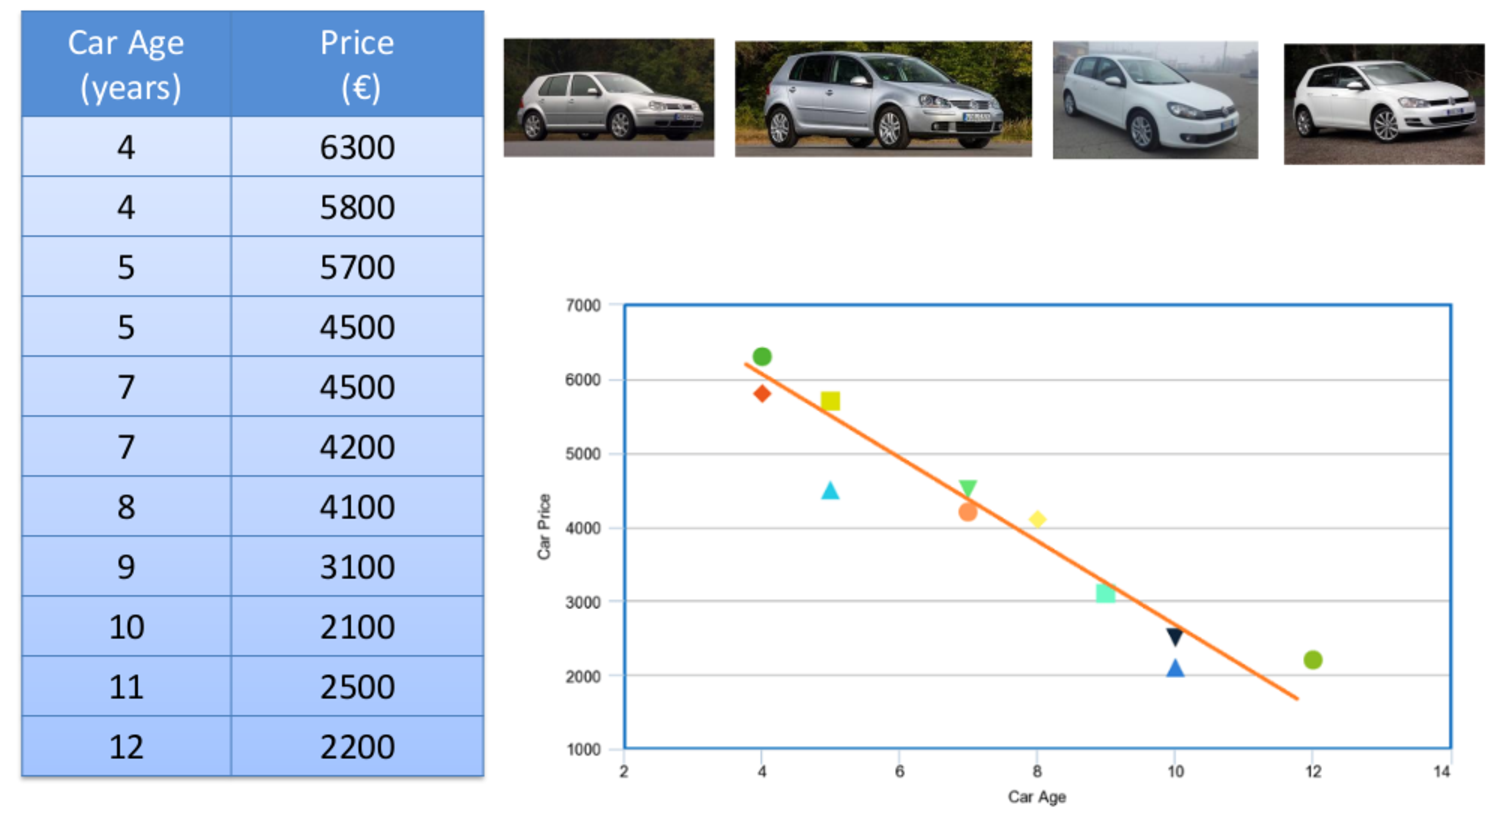
\includegraphics[scale=0.5]{images/linregress_example.pdf}
	\caption{Example of linear regression method}
	\label{fig:ex_lin_regr}
\end{figure}


\section{Least Squares}
The Least Squares is the algorithm that solves the ERM problem for the 
hypothesis class of linear regression predictors with respect to the squared 
loss. The ERM problem with respect to this class, given a training set $S$ and 
using the homogeneous version of $L_d$ is to find the parameters vector that 
minimize the mean-squared error (\ref{eq:mean_squared_err}) between the 
estimated and training values, namely
\[ \underset{\vb{w}}{argmin} L_S(h_{\vb{w}}) = 
\underset{\vb{w}}{argmin}\frac{1}{m}\sum_{i=1}^m\left(\sprod{w}{x_i}-y_i\right)^2
 \]
To solve the problem we calculate the gradient of the objective function and we 
impose it equal to zero:
\[ \frac{2}{m}\sum_{i=1}^m\left(\sprod{w}{x_i}-y_i\right)\vb{x_i}=0 \]
We can rewrite the problem as $A\vb{w}=\vb{b}$ where
\[ 
A=\left(\sum_{i=1}^m\vb{x_i}\vb{x_i^T}\right)\quad\text{and}\quad\vb{b}=\sum_{i=1}^m
y_i\vb{x_i} \] 
If $A$ is invertible then the solution of the ERM problem is 
\[ \vb{w}=A^{-1}\vb{b} \]
Inversion of $A$ is the most expensive operation, from a computational point of 
view. However, the case in which $A$ is not invertible requires a special 
handling (not part of the course).

\section{Polynomial Regression}
Some learning tasks call for nonlinear predictors, such as polynomial 
predictors. Take, for instance, a one dimensional polynomial function of degree 
$n$ that is
\[ p(x)=a_0+a_1x+a_2x^2+\dots +a_nx^n \]
where $(a_0,\dots,a_n)$ is a vector of coefficients of size $n+1$ that we have 
to estimate.\\
One way to learn this class is by reduction to a linear regression problem, 
which we already know how to solve. To translate a polynomial regression 
problem to a linear regression one we define the mapping:
\[ \psi:\mathds{R}\to\mathds{R}^{n+1} \qquad \psi(x)=(1,x,x^2,\dots,x^n) \]
So, we obtain that:
\[ p(\psi(x))=a_0+a_1x+a_2x^2+\dots+a_nx^n=\sprod{a}{\psi(x)} \] 
and we can find the optimal vector coefficients using, for example, the Least 
Squares method.\\
What we have just done is moving to an higher dimensional space, transforming 
the nonlinear problem we were trying to solve in an easier linear one.\\
We also need to notice that however the variables are not independent and the 
optimization can become unstable for large $n$.

\section{Logistic Regression}
In Logistic Regression we learn a family of functions $h$ from $\mathds{R}^d$ 
to the interval $[0,1]$. It is mostly used for classification problems to 
reframe them as regression problem: we can in fact interpret $h(\vb{x})$ as the 
\textit{probability} that 1 is the label of $\vb{x}$.\\
The hypothesis class associated with logistic regression is the composition of 
a \textbf{sigmoid function} $\phi_{sig}:\mathds{R}\to[0,1]$ over the class of 
linear functions $L_d$. In particular, the most used is the \textit{logistic 
function}, represented in picture \ref{fig:logistic_func} and defined as
\[ \phi_{sig}(z)=\frac{1}{1+e^{-z}} \]
\begin{figure}[!h]
	\centering
	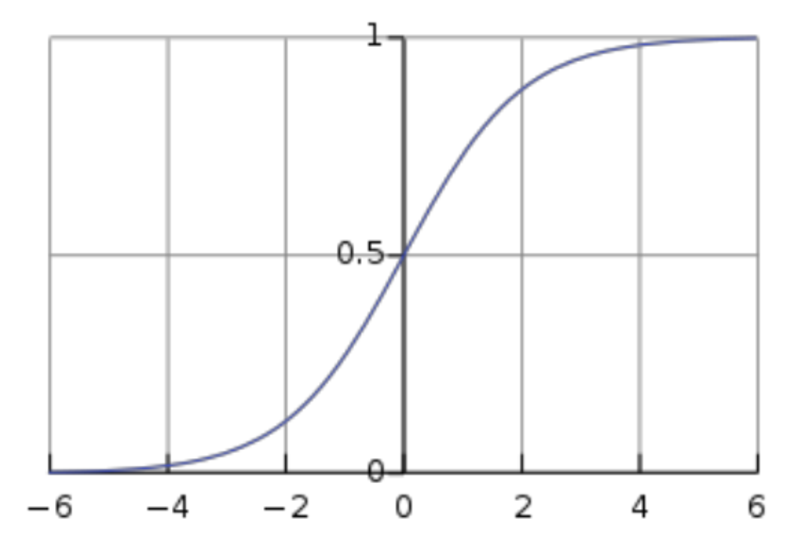
\includegraphics[scale=0.7]{images/logistic_func.pdf}
	\caption{Logistic Function}
	\label{fig:logistic_func}
\end{figure}
Properties:
\begin{itemize}
	\item It is bigger than $1/2$ for positive values and smaller for negative 
	ones.
	\item Tends to 1 for large positive values and to 0 for negative ones.
	\item Can be viewed as a scaled and shifted $sign$ function.
\end{itemize}
The hypothesis class, in the homogeneous case, is
\[ H_{sig}=\phi_{sig}\circ 
L_d=\left\{\vb{x}\to\phi_{sig}\left(\sprod{w}{x}\right):\vb{w}\in\mathds{R}^d 
\right\} \]
Note that when the scalar product $\sprod{w}{x}$ is very large then 
$\phi_{sig}(\sprod{w}{x})$ is close to 1, while when that quantity is very 
small then $\phi_{sig}(\sprod{w}{x})$ is close to 0.\\
Recall that the predictor of the halfspace corresponding to a vector $\vb{w}$ 
is the quantity $sign(\sprod{w}{x})$. Therefore the predictions of the 
halfspace hypothesis and the logistic hypothesis are very similar whenever 
$\abs{\sprod{w}{x}}$ is large. However, when $\abs{\sprod{w}{x}}$ is close to 0 
we have that $\phi_{sig}(\sprod{w}{x})\simeq 1/2$. Intuitively, the logistic 
hypothesis is not sure about the value of the label, so it guessed that is 
$sign(\sprod{w}{x})$ with probability slight to $50\%$. In contrast, the 
halfspace hypothesis always output a deterministic prediction of either 1 or 
-1, even if $\abs{\sprod{w}{x}}$ is very close to 0.\\
Next, we specify a loss function:
\[ \ell\left(h_{\vb{w}},(\vb{x},y)\right)=\log(1+e^{-y\sprod{w}{x}}) \]
Therefore, given a training set $S=(\vb{x_1},y_1),\dots,(\vb{x_m},y_m))$, the 
ERM problem associated with logistic regression is
\[ \underset{\vb{w}\in\mathds{R}^d}{argmin} \frac{1}{m}\sum_{i=1}^m 
\log(1+e^{-y_i\sprod{w}{x_i}}) \]


 \section{Maximum Likelihood Estimation}
The Maximum Likelihood Estimator (MLE) is a statistical approach to a learning 
problem, used to find the parameters that maximize the joint probability o a 
given dataset, assuming a specific parametric probability function.\\
MLE essentially uses a \textit{generative} approach, in which it is assumed 
that the underlying distribution over the data has a specific parametric form.\\
Given a training set $S=((\vb{x_1},y_1),\dots,(\vb{x_m},y_m))$, we assume that 
each $(\vb{x_i},y_i)$ is i.i.d. from some probability distribution 
$\mcl{P}_\theta$ that is characterized by some parameters that we want to 
estimate. Next, we consider the \textit{likelihood} of data (given the 
parameters), i.e. the joint probability of the dataset:
\[ L(S|\theta)=\prod_{i=1}^m\mcl{P}_\theta(\vb{x_i}) \]
Then, to maximize this function, we consider its logarithm: the function $\log$ 
is monotonic, so it will preserve the maximum but it will be also simpler to 
differentiate.
\[ 
\log(L(S|\theta))=\log\left(\prod_{i=1}^m\mcl{P}_\theta(\vb{x_i})\right)=\sum_{i=1}^m\log\left(\mcl{P}_\theta(\vb{x_i})\right)
  \]
At this point, we want to compute the best choice for the parameter $\theta$, 
that is the one that maximize the likelihood function:
\[ \hat{\theta}=\underset{\theta}{argmax}\, L(S|\theta) \]

\subsection{MLE and Logistic Regression}
We can show that MLE solution is equivalent to ERM solution for logistic 
regression.\\
As we know, for logistic regression:
\begin{enumerate}
	\item Assume the training set 
	$S=\left((\vb{x_1},y_1),\dots,(\vb{x_m},y_m)\right)$
	\item 
	$P\left[y_i=1\right]=h_{\vb{w}}(\vb{x_i})=\frac{1}{1+e^{-\sprod{w}{x_i}}}=\frac{1}{1+e^{-y_i\sprod{w}{x_i}}}$
	\item 	
	$P\left[y_i=-1\right]=1-h_{\vb{w}}(\vb{x_i})=\frac{1}{1+e^{\sprod{w}{x_i}}}=\frac{1}{1+e^{-y_i\sprod{w}{x_i}}}$
	\item Likelihood of the training set (joint probability):
	\[ P\left[S|\vb{w}\right]=\prod_{i=1}^m 
	\left(\frac{1}{1+e^{-\sprod{w}{x_i}}}\right) \]
	\[ \log(P\left[S|\vb{w}\right])=-\sum_{i=1}^m 
	\log(1+e^{-y_i\sprod{w}{x_i}}) 
	\]
\end{enumerate}
While the Maximum Likelihood Estimator is:
\[ \underset{\vb{w}}{argmax}\;L(S;\vb{w})=\underset{\vb{w}}{argmax}\; 
\log(P[S|\vb{w}])=\underset{\vb{w}}{argmin}\;\sum_{i=1}^m 
\log(1+e^{-y_i\sprod{w}{x_i}}) \]



\chapter{VC Dimension}
We have seen, in the previous chapters, that a finite class 
($\abs{\mcl{H}}<\infty$) is agnostic PAC learnable. What about infinite 
classes? We would like to understand when infinite classes are learnable and 
also the number of samples that we need to work with.\\ To show that the size 
of the hypothesis class is not the right characterization of its sample 
complexity, we first present a simple example of an infinite-size hypothesis 
class that is learnable.\\

\vspace{0.5cm}
\begin{example}
	Let $\mcl{H}$ be the set of \textit{threshold functions} over the real line, namely $\mcl{H}=\left\{h_a:a\in\mathds{R}\right\}$ where $h_a:\mathds{R}\to\left\{0,1\right\}$ is a function such that $\left\{\begin{aligned}&1\quad\text{if}\quad x<a\\&0\quad\text{otherwise}\end{aligned}\right.$.\\
	Clearly, $\mcl{H}$ is of infinite size, but we can show that $\mcl{H}$ is PAC learnable, using the ERM rule, with sample complexity $m_\mcl{H}(\varepsilon,\delta)\leq\left[\log(2/\delta)/\varepsilon\right]$.
	
	\begin{proof}
		Let $a^*$ be a threshold such that the hypothesis $h^*(x)$ achieves $L_\mcl{D}(h^*)=0$. Let $\mcl{D}_x$ be the marginal distribution over the domain $\mcl{X}$ and let $a_0 < a^* < a_1$ be such that
		\[ \underset{x\sim\mcl{D}_x}{\mathds{P}}\left[x\in(a_0,a^*)\right]= \underset{x\sim\mcl{D}_x}{\mathds{P}}\left[x\in(a^*,a_1)\right]=\varepsilon \]
		Given a training set S, let $b_0=\max\left\{x:(x,1)\in S\right\}$ and $b_1=\min\left\{x:(x,0)\in S\right\}$. Let $b_S$ be a threshold corresponding to ERM hypothesis $h_S$, which implies that $b_S\in(b_0,b_1)$. Therefore, the sufficient condition for $L_\mcl{D}(h_S)\leq\varepsilon$ is that both $b_0\geq a_0$ and $b_1\leq a_1$. In other words):
		\[ \underset{S\sim\mcl{D}^m}{\mathds{P}}\left[L_\mcl{D}(h_S)>\varepsilon\right]\leq \underset{S\sim\mcl{D}^m}{\mathds{P}}\left[b_0<a_0\vee b_1>a_1 \right] \leq\underset{S\sim\mcl{D}^m}{\mathds{P}}\left[b_0<a_0\right]+\leq\underset{S\sim\mcl{D}^m}{\mathds{P}}\left[b_1>a_1\right] \]
		where, in the second disequation, we used the union bound. 
		The event $b_0<a_0$ happens only if all examples in S are not in the interval $(a_0,a^*)$, whose probability mass is defined to be $\varepsilon$, namely:
		\[ \underset{S\sim\mcl{D}^m}{\mathds{P}}\left[b_0<a_0\right]=\leq\underset{S\sim\mcl{D}^m}{\mathds{P}}\left[\forall (x,y)\in S,\; x\notin(a_0,a^*)\right] = (1-\varepsilon)^m \leq e^{-\varepsilon m} \]
		Since we assume $m\geq \log(2/\delta)/\varepsilon$ it follows that the equation is at most $\delta/2$. In the same way it is easy to see that 
		\[ \underset{S\sim\mcl{D}^m}{\mathds{P}}\left[b_1>a_1\right]\leq \frac{\delta}{2} \]
		Combining it with the previous relation we conclude our proof.	
	\end{proof}
\end{example}
\vspace{0.5cm}

We see, therefore, that while finiteness of $\mcl{H}$ is a sufficient condition for learnability, it is not a necessary condition.\\
Before giving the next definitions, let us recall the No Free Lunch theorem and its proof: we have shown that without restricting the hypothesis class, for any learning algorithm, an adversary can construct a distribution for which the learning algorithm will perform poorly, while there is another learning algorithm that will succeed on the same distribution. To proove that, the idea was to select a distribution concentrated on a set C (so a restriction) on which the algorithm fails. Since we are considering distributions that are concentrated on elements of C, we should study $\mcl{H}$ behaves on C.
\begin{definition}(\textbf{Restriction of $\mcl{H}$ to C})\\
	Let $\mcl{H}$ be a class of functions from $\mcl{X}$ to $\left\{0,1\right\}$ and let $C=\left\{c_1,\dots ,c_m\right\}\subset\mcl{X}$. The restriction $\mcl{H}_C$ of $\mcl{H}$ to C is:
	\[ \mcl{H}_C=\left\{\left[h(c_1),\dots ,h(c_m)\right] :h\in\mcl{H}\right\} \]
	where we represent each function from C to $\left\{0,1\right\}$ as a vector in $\left\{0,1\right\}^\abs{C}$.
\end{definition}
If the restriction of $\mcl{H}$ in C is the set of all functions from C to $\left\{0,1\right\}$, then we say that $\mcl{H}$ \textit{shatters} the set C. Formally
\begin{definition}(\textbf{Shattering})\\
	A hypothesis class $\mcl{H}$ shatters a finite set $C\subset\mcl{X}$ if the restriction of $\mcl{H}$ to C is the set of all functions from C to $\left\{0,1\right\}$, that is $\abs{\mcl{H}_C} =2^\abs{C}$.
\end{definition}
Getting back to the construction of an adversarial distribution as in the proof of the No-Free-Lunch theorem, we see that whenever some set C is shattered by $\mcl{H}$, the adversary is not restricted by $\mcl{H}$, as they can construct a distribution over C based on any target function from C to $\left\{0,1\right\}$, while still maintaining the realizability assumption. This immediately yields:
\begin{corollary}
	Let $\mcl{H}$ be a hypothesis class of functions from $\mcl{X}$ to $\left\{0,1\right\}$. Let $m$ be a training set size. Assume that there exist a set $C\subset\mcl{X}$ of size $2m$ that is shattered by $\mcl{H}$. Then for any learning algorithm A there exist a distribution $\mcl{D}$ over $\mcl{X}\times\left\{0,1\right\}$ and a predictor $h\in\mcl{H}$ such that $L_d(h)=0$ but with probability at least 1/7 over the choice of S we have that $L_\mcl{D}(A(S))\geq 1/8$.
	\label{cor:NFL_shattering}
\end{corollary}
This corollary tells us that if $\mcl{H}$ shatters some set C of size $2m$ then we cannot learn $\mcl{H}$ using $m$ examples.
\begin{definition}(\textbf{VC-dimension})\\
	The VC-dimension of an hypothesis class $\mcl{H}$, denoted $VCdim(\mcl{H})$, is the maximal size of a set $C\subset\mcl{X}$ that can be shattered by $\mcl{H}$. If $\mcl{H}$ can shatter sets of arbitrarily large size we say that $\mcl{H}$ has infinite VC-dimension.
\end{definition}

Notice that:
\begin{itemize}
	\item If $\mcl{H}$ is a finite class, for any set $C$ we have $\abs{\mcl{H}_C}\leq\abs{H}$ and thus C cannot be shattered if $\abs{\mcl{H}}\leq2^\abs{C}$. This implies that $VCdim(\mcl{H})\leq\log_2(\abs{\mcl{H}})$.
	\item If $\mcl{H}$ has an infinite VC-dimension it is not PAC learnable: as a consequence of the corollary \ref{cor:NFL_shattering}, there will always exist a subset of size $2m$ that is shattered for any $m$.
\end{itemize}

To show that $VCdim(\mcl{H})=d$ we need to show that:
\begin{itemize}
	\item[1.] $VCdim(\mcl{H})\geq d$: there exists a set $C$ of size $d$ that is shattered by $\mcl{H}$.
	\item[2.] $VCdim(\mcl{H})\leq (d+1)$: every set $C$ of size $d+1$ is not shattered by $\mcl{H}$.
\end{itemize}

\begin{example} (Threshold functions)\\
	Let $\mcl{H}$ be the class of threshold functions over $\mathds{R}$. Take a set $C=\left\{c_1\right\}$. Now, if we take $a=c_1+1$, then we have $h_a(c_1)=1$, and if we take $a=c_1-1$, then we have $h_a(c_1)=0$. Therefore, $\mcl{H}_C$ is the set of all the functions from $C$ to $\left\{0,1\right\}$, and $\mcl{H}$ shatters $C$. Now let's take a set $C=\left\{c_1,c_2\right\}$, where $c_1\leq c_2$. No $h\in\mcl{H}$ can account for the labeling $(0,1)$, because any threshold that assign the label 0 to $c_1$ must assign the label 0 to $c_2$ as well. Therefore not all functions from $C$ to $\left\{0,1\right\}$ are included in $\mcl{H}_C$; hence $C$ is not shattered by $\mcl{H}$.\\
	So, we just proved that an arbitrary set $C=\left\{c_1\right\}$ is shattered by $\mcl{H}$ (where $\mcl{H}$ is the class of threshold functions over $\mathds{R}$); therefore $VCdim(\mcl{H})\geq 1$. At the same time, an arbitrary set $C=\left\{c_1,c_2\right\}$ is not shattered by $\mcl{H}$. So we can conclude that $VCdim(\mcl{H})=1$.
\end{example}

\begin{example} (Intervals)\\
	Let $\mcl{H}$ be the class of intervals over $\mathds{R}$, namely $\mcl{H}=\left\{h_{a,b}:a,b\in\mathds{R},a<b\right\}$, where $h_{a,b}:\mathds{R}\to\left\{0,1\right\}$ is a functions that is 1 for $x\in(a,b)$ and 0 otherwise. Let's take the set $C=\left\{1,2\right\}$. Then, $\mcl{H}$ shatters $C$ and therefore $VCdim(\mcl{H})\geq 2$. Now let's make an arbitrary set $C=\left\{c_1,c_2,c_3\right\}$ and assume without loss of generality that $c_1\leq c_2\leq c_3$. Then, the labeling (1,0,1) cannot be obtained by an interval, and therefore $\mcl{H}$ does not shatter $C$. We therefore conclude that $VCdim(\mcl{H})=2$.
\end{example}

\begin{example} (Axis aligned rectangles)\\
	Let $\mcl{H}$ be the class of axis aligned rectangles, formally: $\mcl{H}=\left\{h_{(a_1,a_2,b_1,b_2)}:a_1\leq a_2 \text{ and } b_1\leq b_2 \right\}$, where 
	\[ h_{(a_1,a_2,b_1,b_2)} = \left\{\begin{aligned}&1\quad if\; a_1\leq x_1\leq a_2 \text{ and } b_1\leq x_2\leq b_2\\ &0\quad\text{otherwise}\end{aligned}\right. \]
	
	As can be seen in figure \ref{fig:axis_al_rect}, it is easy to find a set of 4 points that are shattered, so $VCdim(\mcl{H})\geq 4$. 
	\begin{figure}[!h]
		\centering
		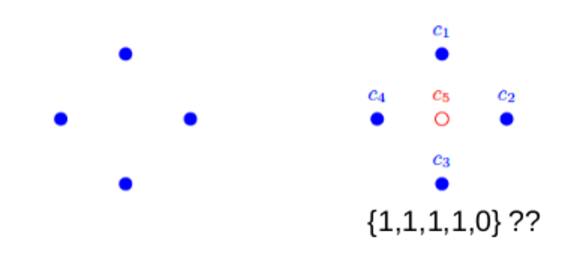
\includegraphics[scale=1]{images/axis_aligned_rectangles.pdf}
		\caption{Left: 4 points are shattered by axis aligned rectangles. Right: any axis aligned rectangle cannot label $c_5$ by 0 and the rest of the points by 1}
		\label{fig:axis_al_rect}
	\end{figure}
	Now let's consider any set $C\in\mathds{R}^2$ of 5 points from which we are gonna take the leftmost, the rightmost, the highest and the lowest one. Without loss of generality, denote $C=\left\{c_1,\dots,c_5\right\}$ and let $c_5$ be the point that was not selected. It is impossible to obtain the label (1,1,1,1,0) by any axis aligned rectangle, because such rectangle must contain $c_1,\dots,c_4$, but at the same time must contain $c_5$ too, because its coordinates are within the intervals defined by the selected points. So this $C$ is not shattered by $\mcl{H}$, and therefore $VCdim(\mcl{H})=4$.
\end{example}

\begin{example} (\textbf{VC dimension of halfspaces hypothesis class})\\
	We want to prove that the VC dimension of the class of homgeneous 
	halfspaces in $\mathds{R}^d$ is $d$.
	\begin{itemize}
		\item $VCdim(\mcl{H})\geq d$: I have to find at least one set of size 
		$d$ that is shattered by $\mcl{H}$. For this reason I consider the set 
		of vectors $\vb{e}_1,\dots,\vb{e}_d$, that are the vectors of the 
		canonical base in $\mathds{R}^d$: this set is shattered by the class 
		$\mcl{H}$. In fact, for labeling $y_1,\dots,y_d$, and setting 
		$\vb{w}=(y_1,\dots,y_d)$, then $sprod{w}{e_i}=y_i$ for all $i$.
		\item $VCdim(\mcl{H})\leq d$: I have to show that every possible set of 
		size $d+1$ cannot be shattered. Let's consider the generic $d+1$-set 
		$\vb{x}_1,\dots,\vb{x}_{d+1}$; these vectors, as we known from 
		geometry, are linearly dependent, i.e. there exists a set of parameters 
		$\alpha_1,\dots,\alpha_{d+1}$ (not all zeros) such that 
		$\sum_{i=1}^{d+1}\alpha_i\vb{x_i}=0$. So, if I define the two sets 
		$I=\left\{i:\alpha_i>0\right\}$ and $J=\left\{j:\alpha_j<0\right\}$, at 
		least one of these is not empty. Let us first assume that both of them 
		are nonempty, then:
		\[ \sum_{i\in I}\alpha_i\vb{x}_i = \sum_{j\in J}\abs{\alpha_j}\vb{x}_j 
		\] 
		Now suppose that $\vb{x}_1,\dots,\vb{x}_{d+1}$ are shattered by the 
		class of homogeneous halfspaces. Then, there must exist a vector 
		$\vb{w}$ such that $\sprod{w}{x_i}>0$ for all $i\in I$ while 
		$\sprod{w}{x_j}<0$ for all $j\in J$. It follows that
		\[ 0<\sum_{i\in I}\alpha_i\sprod{x_i}{w}=\sprod{\sum_{i\in 
		I}\alpha_i\vb{x_i}}{w}=\sprod{\sum_{j\in 
		J}\abs{\alpha_j}\vb{x_j}}{w}=\sum_{j\in 
		J}\abs{\alpha_j}\sprod{x_j}{w}<0 \]
		which leads to a contradiction. Finally, if $J$ (respectively, $I$) is 
		empty, then the right-most (respectively, left-most) inequality should 
		be replaced by an equality, which still leads to contradiction.
	\end{itemize}
	Also, the VC dimension of the class of nonhomogeneous halfspaces in 
	$\mathds{R}^d$ is $d+1$.
\end{example}

Care, that the VC dimension does not always correspond to the number of 
parameters!
\begin{example}
	We can look for example at the class 
	$\mcl{H}=\left\{h_\theta:\theta\in\mathds{R}\right\}$, 
	$h_\theta:\mcl{X}\to\left\{0,1\right\}$ $h_\theta=\left[0.5\sin(\theta 
	x)\right]$.\\
	It can be proved that $\mcl{H}$ has infinite VC dimension.
	\begin{figure}[!h]
		\centering
		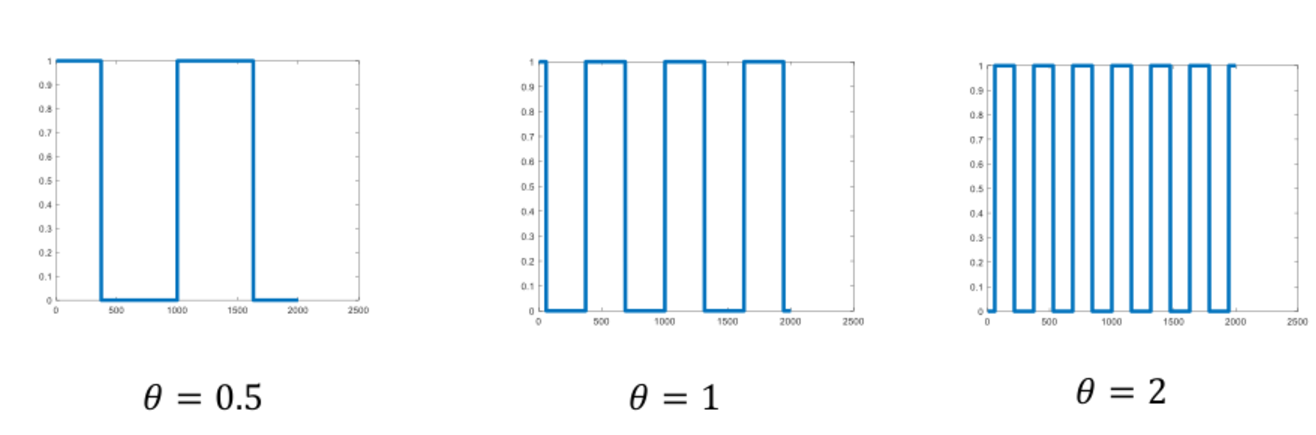
\includegraphics[scale=0.6]{images/ex_infty_VCdim.pdf}
		\caption{Example of a hypothesis class with infinity VC-dimension}
	\end{figure}
\end{example}

\section{Fundamental Theorem of Statistical Learning}
We have already shown that a class of infinite VC-dimension is not learnable; 
however, the opposite statement is also true, as guarantee by the following 
theorem.
\begin{theorem} (\textbf{The Fundamental Theorem of Statistical Learning})\\
	Let $\mcl{H}$ be an hypothesis class of function from a domain $\mcl{X}$ to 
	$\left\{0,1\right\}$ and let the loss function be the 0-1 loss. Then, the 
	following are equivalent:
	\begin{enumerate}
		\item $\mcl{H}$ has the uniform convergence property.
		\item Any ERM rule is a successful agnostic PAC learner for $\mcl{H}$.
		\item $\mcl{H}$ is agnostic PAC learnable.
		\item $\mcl{H}$ is PAC learnable.
		\item Any ERM rule is a successful PAC learner for $\mcl{H}$.
		\item $\mcl{H}$ has a finite VC-dimension.
	\end{enumerate}
\label{th:fundamental_statistical_learning}
\end{theorem} 
Not only does the VC-dimension characterize PAC learnability; it even 
determines the sample complexity, as can be seen in the next theorem.
\begin{theorem} (\textbf{The Fundamental Theorem of Statistical Learning - 
Quantitative version})\\
	Let $\mcl{H}$ be an hypothesis class of function from a domain $\mcl{X}$ to 
	$\left\{0,1\right\}$ and let the loss function be the 0-1 loss. Assume that 
	$VCdim(\mcl{H})=d<\infty$. Then, there are absolute constants $C_1,C_2$ 
	such that:
	\begin{enumerate}
		\item $\mcl{H}$ has the uniform convergence property with sample 
		complexity
		\[ C_1\frac{d+\log(1/\delta)}{\varepsilon^2}\leq 
		m_{\mcl{H}}^{UC}(\varepsilon,\delta)\leq 
		C_2\frac{d+\log(1/\delta)}{\varepsilon^2} \]
		\item $\mcl{H}$ is agnostic PAC learnable with sample complexity 
		\[ C_1\frac{d+\log(1/\delta)}{\varepsilon^2}\leq 
		m_{\mcl{H}}(\varepsilon,\delta)\leq 
		C_2\frac{d+\log(1/\delta)}{\varepsilon^2} \]
		\item $\mcl{H}$ is PAC learnable with sample complexity
		\[ C_1\frac{d+\log(1/\delta)}{\varepsilon}\leq 
		m_{\mcl{H}}(\varepsilon,\delta)\leq 
		C_2\frac{d\log(1/\varepsilon)+\log(1/\delta)}{\varepsilon} \]
	\end{enumerate}
\end{theorem}


\chapter{Model selection and validation}
When approaching some practical problem, we usually can think of several 
algorithms that may yield a good solution, each of which might have several 
parameters. How can we choose the best algorithm for the particular problem at 
hand? And how do we set the algorithm’s parameters? This task is often called 
\textbf{model selection}.\\
The most used approaches are the \textbf{Structral Risk Minimization} (SRM), 
that is not part of the course, and using a \textbf{validation set}.\\

\section{Validation Set}
The basic idea behind this approach is to partition the training data into two 
sets, one to be used to train all the candidate models, and the other to decide 
which of them yields the best results.\\
In model selection tasks, we try to find the right balance between 
approximation and estimation errors. More generally, if our learning algorithm 
fails to find a predictor with a small risk, it is important to understand 
whether we suffer from overfitting or underfitting.\\
We would often like to get a better estimation of the true risk of the output 
predictor of a learning algorithm. So far we have derived bounds on the 
estimation error of a hypothesis class, which tell us that for all hypotheses 
in the class, the true risk is not very far from the empirical risk. However, 
these bounds might be loose and pessimistic, as they hold for all hypotheses 
and all possible data distributions. A more accurate estimation of the true 
risk can be obtained by using some of the training data as a validation set, 
over which one can evalutate the success of the algorithm’s output predictor.
The only price to pay with this method is just part of the training data.\\

So, let's assume that we have picked a predictor $h$ (for example by ERM rule); 
let $V$ be a set of $m_\nu$ samples used as validation set, and let $L_V$ be 
the loss (in $[0,1]$) computed on this set; then, using the Hoeffding 
Inequality (\ref{lem:Hoeffding}), we obtain the following theorem:
\begin{theorem}
	For every $\delta\in(0,1)$, with probability of at least $1-\delta$ over 
	the choice of the validation set $V$ we have:
	\[ 
	\abs{L_V(h)-L_\mcl{D}(h)}\leq\sqrt{\frac{\log(\frac{2}{\delta})}{2m_\nu}} \]
\label{th:validation_theorem}
\end{theorem}
It can be useful to notice that the bound guaranteed from the previous theorem 
does not depend on the algorithm or on the training set used to construct the 
predictor, and also it is tighter than the "usual" bounds. The reason is that 
this bound is independent from the way the predictor was generated.\\
Let's compare, for example, the error on a predictor $h$ obtained by applying 
ERM predictor with respect to a class with VC-dimension $d$, over a training 
set of $m$ samples, that is given by the Fundamental Theorem of Statistical 
Learning (\ref{th:fundamental_statistical_learning}), and the bound imposed by 
\ref{th:validation_theorem}:\\
\vspace{0.5cm}
\begin{figure}[!h]
	\begin{minipage}{0.5\textwidth}
		\[ L_\mcl{D}(h)\leq L_S(h)+\sqrt{C\frac{d+\log(1/\delta)}{m}} \]
		\centering
		\vspace{0.3cm}
		From fundamental theorem
	\end{minipage}
	\begin{minipage}{0.5\textwidth}
		\[ L_\mcl{D}(h)\leq L_V(h)+\sqrt{\frac{\log(2/\delta)}{2m_\nu}} \]
		\centering
		\vspace{0.3cm}
		With validation set
	\end{minipage}
\end{figure}

Therefore, taking $m_\nu$ at least at the same order of $m$, we obtain an 
estimate that is more accurate by a factor that depends on the VC-dimension.\\
However, since the algorithm haven't seen the validation set yet, we are 
protected from the risk of overfitting.\\


\section{Validation for Model Selection}
Validation can be naturally used for model selection.\\
\begin{itemize}
	\item We first have to train different algorithms (or the same algorithm 
	but with different parameters) on the training set, obtaining a set of ERM 
	predictors $\mcl{H}=\left\{h_,h_2,\dots,h_r \right\}$.
	\item Then, we have to choose the predictor that minimizes the error on the 
	validation set. In other words, we apply the ERM predictor over the 
	validation set.
	\item This process is very similar to learning a finite hypothesis class. 
	The only difference is that $\mcl{H}$ is not fixed ahead of time but rather 
	depends on the training set. However, since the validation set is 
	independent from the training set we get that it is also independent from 
	$\mcl{H}$ and therefore the same techniques we used to derive bounds for 
	finite hypothesis class holds here as well.
\end{itemize}
Combining theorem $\ref{th:validation_theorem}$ with union bound, in 
particular, we obtain the 
following theorem:
\begin{theorem}
	Let $\mcl{H}=\left\{h_1,\dots,h_r\right\}$ be an arbitrary set of 
	predictors and assume that the loss function is in $[0,1]$. Assume that a 
	validation set $V$ of size $m_\nu$ is sampled indipendent from $\mcl{H}$. 
	Then, with probability of at least $1-\delta$ over the choice of $V$ we have
	\[ \forall 
	h\in\mcl{H},\;\abs{L_\mcl{D}(h)-L_V(h)}\leq\sqrt{\frac{\log(2\abs{H}/delta)}{2m_\nu}}
	 \]
\end{theorem}
This theorem essentially tells us that the error on the validation set 
approximates the true error as long as $\mcl{H}$ is not too large (too many 
methods can bring to overfitting).\\
\vspace{0.5cm}
\begin{example}
	To illustrate how validation is useful we exploit against the following 
	example in figure \ref{fig:ex_val}: we have a training set, made by the 
	black points, that has been 
	fitted with ERM polynomials of degree 2,3 and 10. But this time we also 
	despict an additional validation set (white points): as can be seen, the 
	polynomial of degree 10 has minimal training error, yet the polynomial of 
	degree 3 has the minimal validation error, and hence it will be chosen as 
	best model.
	\begin{figure}[!h]
		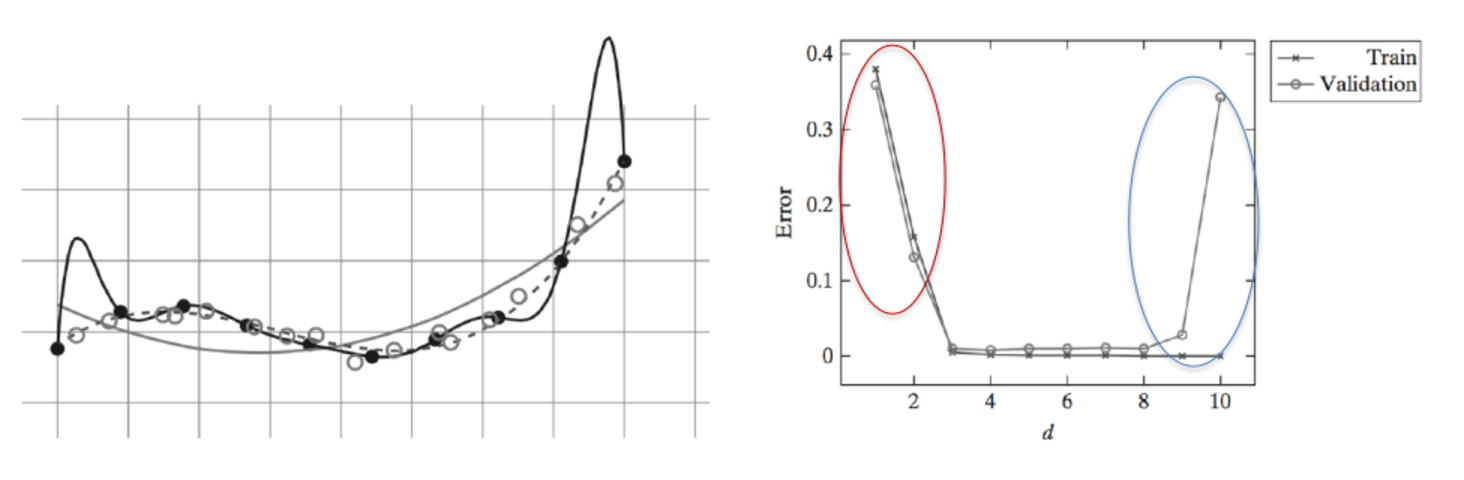
\includegraphics[scale=0.7]{images/ex_validation_set.pdf}
		\caption{Example of Validation efficiency}
		\label{fig:ex_val}
	\end{figure}
	The figure on the right is called \textbf{Model-Selection Curve}, and shows 
	the training error and the validation error as a function of the complexity 
	of the model considered (in this case the polynomial fitting). As can be 
	shown, the training error is monotonically decreasing as we increase the 
	polynomial degree (which is the complexity of the model, in this case), 
	while, on the other hand, the validation error first decreases but then 
	starts to increase, which indicates that we are starting to suffer from 
	overfitting.\\
	However, it is always useful to compute both training and validation error 
	and compare it. If they are close, this means that the algorithm works on 
	training data in the same way he does on the real world.
\end{example}

\subsection{Grid Search for Multiple Parameters}
What happen when we have to estimate one (or more) parameters with value in 
$\mathds{R}$?\\
A possible way to solve this problem is starting with a rough grid of values 
and and plot the corresponding model-selection curve. On the basis of the 
curve, we should zoom into the correct (where "correct" is intended respect to 
our problem) region and start again the procedure with a finer grid. However, 
this research trough the grid does not always find the global optimal solution 
for our parameters, but it can give a reasonable approximation.

\subsection{Train-Validation-Test Split}
In most practical applications, we split the available examples in 3 sets. The 
first, and bigger one, is used for training the algorithm, while the second one 
is used as a validation set to decide which of our hypothesis is the best to 
describe our model. After that, we test the performances of the output 
predictor on the third set, and the number obtained is used as an estimator of 
the true error of the learned predictor.\\
Important: the test set is not involved in the choice of the best predictor 
and, if for some reason we decide to change our best hypothesis, this test set 
cannot be used again to estimate the true error.

\section{K-Fold Cross Validation}
The validation procedure described so far assumes that data is plentiful and 
that we have the ability to sample a fresh validation set. But in reality data 
are often scarce, and we would not "waste" data on validation. The k-fold cross 
validation technique is designed to give an accurate estimate of the true error 
without wasting too much data.\\
In this procedure, the original training set is partitioned into $k$ subsets 
(\textit{folds}) of size $m/k$. For each fold, the algorithm is trained on the 
set built from the union of the other folds, and then the error of its output 
is estimated using the starting fold. The final estimate of the true error is 
computed as the average of the values found for each fold. A schematic 
representation of the technique is figure \ref{ex:5_foldcross}.\\
\begin{figure}[!h]
	\centering
	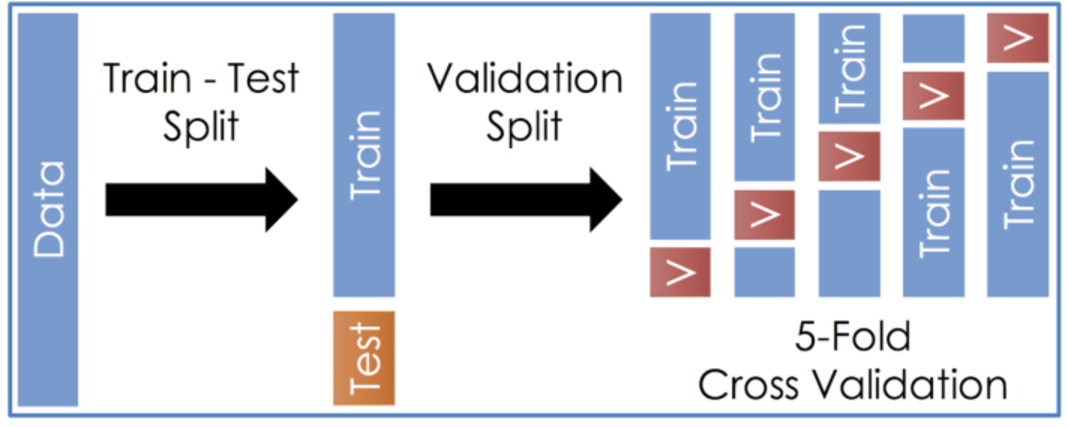
\includegraphics[scale=0.6]{images/5_fold_cross_validation.pdf}
	\caption{Scheme of a 5-Fold Cross Validation}
	\label{ex:5_foldcross}
\end{figure}
K-Fold Cross Validation is often used for model selection: in this case after 
selecting the model, the final hypothesis is obtained from training on the 
entire training set. A pseudo-code of the technique used for model selection is 
given in box \ref{box:k_fold}: the procedure receives an input training set 
$S$, a set 
of possible parameter values $\Theta$, the number of folds $k$ and a learning 
algorithm, and outputs the best parameter as well as the hypothesis trained by 
this parameter on the entire training set.\\

\begin{tcolorbox}
	\begin{center}
		\textbf{k-Fold Cross Validation for Model Selection}
	\end{center}
	\textbf{Input:}\\
	\-\ training set $(\vb{x}_1,y_1),\dots,(\vb{x}_m,y_m)$\\
	\-\ set of parameter values $\Theta$\\
	\-\ learning algorithm $A$\\
	\-\ number of folds $k$\\
	 
	\textbf{Partition:} $S$ in $S_1,S_2,\dots,S_k$\\
	
	\textbf{foreach} $\theta\in\Theta$\\
	\-\ for $i=1,\dots,k:$\\
	\-\ \quad $h_{i,\theta}=A(S/S_i;\theta)$ \qquad\qquad $\backslash*$ 
	removing the i-th fold $*\backslash$\\
	\-\ $error(\theta) = \frac{1}{k}\sum_{i=1}^k L_{S_i}(h_{i,\theta})$\\
	
	\textbf{output:}\\
	\-\ $\theta^* = argmin_\theta\left[error(\theta)\right]$\\
	\-\ $h_{\theta^*} = A(S;\theta^*)$
\label{box:k_fold}
\end{tcolorbox}

\section*{Error Decomposition}
Let's recall all the error we have define until now:
\begin{itemize}
	\item $L_\mcl{D}(h^*)$ is the \textit{approximation error}, i.e. the true 
	error over the best hypothesis in $\mcl{H}$.
	\item $L_\mcl{D}(h_S)-L_\mcl{D}(h^*)$ is the \textit{estimation error}, 
	i.e. the difference between the true error of the best hypothesis in 
	$\mcl{H}$ and the true error of the ERM solution.
	\item $L_S(h_S)$ is the \textit{training error} i.e. the empirical error of 
	the ERM solution on the training set $S$.
	\item $L_V(h_S)$ is the \textit{validation error} i.e. the error over the 
	validation set $V$ of the ERM solution.
\end{itemize}
Thank to this we can decompose the true error of the ERM solution as follows 
(and that we have already described in section \ref{sec:err_dec}):
\[ L_\mcl{D}(h_S) = L_\mcl{D}(h^*) L_\mcl{D}(h_S)-L_\mcl{D}(h^*) \]
As well with the training and the validation error:
\[ L_\mcl{D}(h_S) = (L_\mcl{D}(h_S)-L_V(h_S)) + (L_V(h_S)-L_S(h_S)) + L_S(h_S) 
\]
However, it is more difficult to estimate the approximation error of the class, 
and so we give such an error decomposition, that let us to focus on training 
and validation error. The first term of this decomposition, 
$L_\mcl{D}(h_S)-L_V(h_S)$, can easily bounded using theorem 
\ref{th:validation_theorem}; when the second one, $L_V(h_S)-L_S(h_S)$, tends to 
be large we can say that our algorithm suffers from "overfitting"; when the 
last term, the empirical risk $L_S(h_S)$, is large, we can say that this is a 
case of "underfitting". 


\section{When Learning Fails}
Consider the following scenario: you were given a learning task and have 
approached it with a choice of an hypothesis class, a learning algorithm, and 
parameters. You used a validation set to tune the parameters and tested the 
learned predictor on a test set. The test result, unfortunately, turn out to be 
unsatisfactory. What went wrong, then, and what should you do next?\\
There are many elements that can be changed to gain better results, for example:
\begin{itemize}
	\item Get a larger sample
	\item Change the hypothesis class (enlarging it, reducing it or completely 
	changing the parameters or the class itself)
	\item Change the feature representation of the data
	\item Change the optimization algorithm used to apply the learning rule
\end{itemize}
In order to find the best remedy, it is essential first to understand the cause 
of the bad performance. Remember that the approximation error does not depend 
on the sample size or on the algorithm being used, but only on the distribution 
$\mcl{D}$ and on the hypothesis class $\mcl{H}$. Therefore, if the 
approximation error is large, it will not help us to enlarge the training set 
size, and it also does not make sense to reduce the hypothesis class. What can 
be beneficial in this case is to enlarge the hypothesis class or completely 
change it (if we have some alternative prior knowledge in the form of a 
different hypothesis class). The estimation error of the class, instead, does 
depend on the sample size. Therefore, if we have large estimation error we can 
make an effort to obtain more training examples. We can also consider reducing 
the hypothesis class. However, it doesn't make sense to enlarge the hypothesis 
class in that case.\\
One possible way to distinguish between over and underfitting and estimate di 
approximation error $L_\mcl{D}(h^*)$ is by plotting the so called 
\textit{learning curves}. To produce a learning curve we train the algorithm on 
prefixes of data of increasing sizes (for example we can first train it on 
$10\%$ of data, then on $20\%$ and so on). For each of these data subgroup we 
calculate the training error and the validation one (on a predefine validation 
set), and then we plot it together as in figure \ref{fig:learning_curves}.
\begin{figure}[!h]
	\centering
	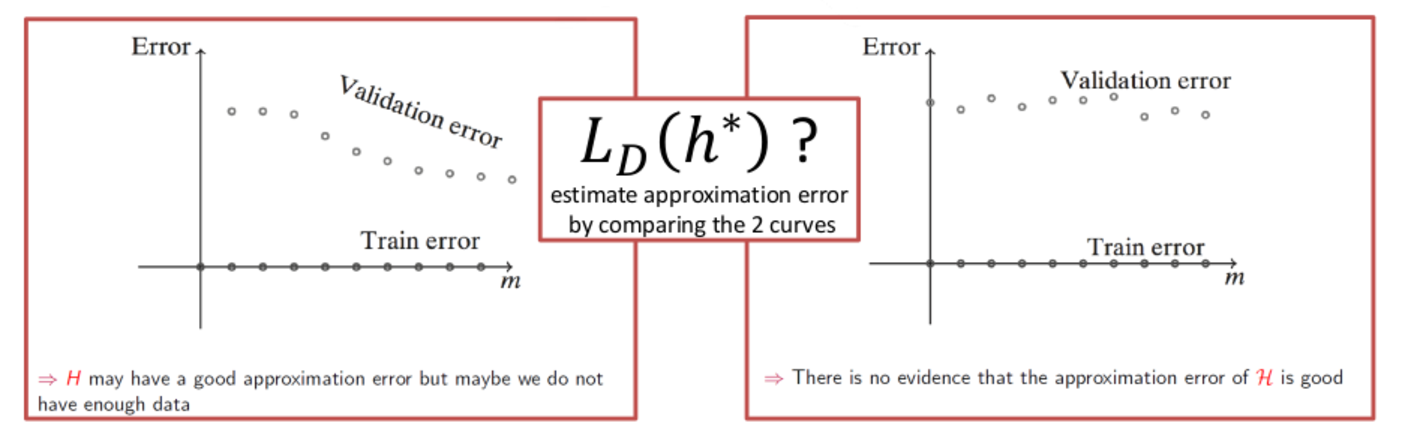
\includegraphics[scale=0.7]{images/learning_curves.pdf}
	\caption{Example of learning curves. Left: scenario in which the number of 
	examples is always smaller than the VC-dimension of the problem. Right: 
	scenario in which the approximation error is zero and the number of 
	examples is larger than the VC-dimension.}
	\label{fig:learning curves}
\end{figure}
Such curves help us to distinguish the two aforementioned scenarios. In 
general, as long as the approximation error is greater than zero we expect the 
training error to grow with the sample size, as a larger amount of data points 
makes it harder to provide an explanation for all of them. On the other hand, 
the validation error tends to decrease with the increase in the sample size. If 
the VC-dimension is finite, when the sample size goes to infinity, the 
validation and train errors converge to the approximation error.\\

To summarize the discussion, the following steps should be applied:
\begin{enumerate}
	\item If learning involves parameter tuning, plot the model-selection curve 
	to make sure that they have been tuned appropriately.
	\item If the training error is excessively large, consider enlarging the 
	hypothesis class, completely change it, or change the feature 
	representation of the data.
	\item If the training error is small, plot learning curves and try to 
	deduce from them if the problem is the estimation error or the 
	approximation one.
	\item If the approximation error seems to be small enough, try to obtain 
	more data. If it is not possible, consider reducing the complexity of the 
	hypothesis class.
	\item If the approximation error seems to be large as well, try to change 
	the hypothesis class or the feature representation of the data completely.
\end{enumerate}


\chapter{Regularization and Stability}

In this chapter we are gonna introduce a new learning paradigm, called 
\textbf{Regularized Loss Minimization}, or RLM, for short. In RLM we minimize 
the sum of the empirical risk and a regularization function, that quantifies 
the complexity of hypotheses. Another view or regularization is as a 
\textbf{stabilizer} of the learning algorithm. An algorithm is considered 
stable if a slight change of the input does not change the output much.

\section{Regularized Loss Minimization}
RLM is a learning rule in which we jointly minimize the empirical risk and a 
regularization function. Formally, given an hypothesis $h$, characterized by a 
vector of parameters $\vb{w}=(w_1,\dots,w_d)^T\in\mathds{R}^d$ (for example the 
coefficients of a linear regression or the weights of a neural network), a 
\textit{regularization function} is a map $R:\mathds{R}^d\to\mathds{R}$, 
function of $\vb{w}$, for which the RLM rule outputs an hypothesis in 
\[ \underset{\vb{w}}{argmin}\left(L_S(\vb{w})+R(\vb{w})\right) \]  
where $L_S(\vb{w})$ is the standard loss and $R(\vb{w})$ is a regularization 
term that measures, in some way, the "complexity" of the found solution, it 
balances between a low empirical risk and aiming at less complex hypotheses.\\
There are many possible regularization functions that one can use, reflecting 
some prior knowledge about the problem. One of the most simple regularization 
functions (that make use of the $\ell_2$ norm), known as \textbf{Tikhonov 
Regularization}, is
\[ R(\vb{w})=\lambda\norm{\vb{w}}^2=\lambda\sum_{i=1}^d w_i^2 \]
where $\lambda>0$ is a scalar.\\
Using this formula, the learning rule becomes
\[ 
A(S)=\underset{\vb{w}}{argmin}\left(L_S(\vb{w})+\lambda\norm{\vb{w}}^2\right) \]
One interpretation sees the norm $\norm{\vb{w}}^2$ as a measurement of the 
complexity of the hypothesis class defined by the vector $\vb{w}$, and the 
parameter $\lambda$ as a coefficient used to control the trade-off between a 
low empirical risk and an high complexity (risk of overfitting).

\subsection{Ridge Regression}










\end{flushleft}
\end{document}
